\chapter{Explainable Anomaly Detection for Vehicle Fuel Consumption: Explanation Generation and Evaluation Using Prior Domain Knowledge}\label{chap:6-fleet-xai}

In this chapter, we focus on the second real use case within this thesis for Explainable Artificial Intelligence (XAI) for real-world applications. Specifically for this use case, the data feeds where anomalies need to be detected and explained are related to vehicle fuel consumption data. Thus, our aim is to generate explanations that indicate why a specific vehicle has an anomalous fuel consumption, which features are causing it, how much do they impact on the extra fuel usage, and how much fuel could be saved if their values changed to a particular reference.

For that, we propose a methodology for generating explanations over the output of an unsupervised anomaly detection model, which shows in terms of feature relevance how much fuel could be saved if certain features changed their value to a specific reference. This methodology includes the usage of prior domain knowledge for both adjusting the explanations according to it, as well as evaluating them against it in order to see if they are aligned. It also includes the usage of other XAI-specific metrics for comparing different XAI alternatives in terms of other aspects. With that, with this chapter, we continue the research from \hyperref[chap:4-rule-extraction]{Chapter} \ref{chap:4-rule-extraction} in terms of XAI-metrics, and the research from \hyperref[chap:5-comms-xai]{Chapter} \ref{chap:5-comms-xai} in terms of using domain knowledge, proposing and evaluating a solution that aims to answer the main hypothesis of this thesis by addressing the two sub-hypothesis beneath it: the usage of XAI techniques for generating explanations over the output of unsupervised anomaly detection algorithms, including the evaluation of the results with XAI-specific metrics (\textbf{H1}), and the combination of XAI techniques with prior domain knowledge both within the explanation generation and within the metric evaluations (\textbf{H2}).

The contributions of this chapter are related to \textbf{C2.2}, introduced in \hyperref[sec:Hypotheses]{Section} \ref{sec:Hypotheses} within the \hyperref[chap:3-objetives]{Chapter} \ref{chap:3-objetives}, and appear in our submitted paper \parencite{barbado2021anomaly} and in our registered patent \parencite{patent2020fleet}.

We divide this chapter in the following sections. \hyperref[sec:ch6-IntroFleet]{Section} \ref{sec:ch6-IntroFleet} introduces the problem and gives the context for our proposals. \hyperref[sec:ch6-method]{Section} \ref{sec:ch6-method} describes our XAI method for explaining anomalies within the context of vehicle fuel consumption, including the proposal for combining those explanations with prior knowledge, and the different XAI metrics for measuring both general explainability aspects, as well as the alignment of the explanations to that prior knowledge. In \hyperref[sec:ch6-evaluation]{Section} \ref{sec:ch6-evaluation} we present the empirical evaluation carried out with our proposal. Finally, \hyperref[sec:ch6-conclusion]{Section} \ref{sec:ch6-conclusion} presents a summary of the conclusions for this chapter.

% Cambiar en COMMS (CAP3) para decir que solo evalua H2, y que asi como CH4 evalua H1, y CH5 evalua H2, aqui pasamos a evaluar tanto H1 como H2.

\section{Introduction}\label{sec:ch6-IntroFleet}
Combining Advanced Analytics techniques together with IoT (Internet of Things) data offers many possibilities for finding and extracting relevant insights for business decisions. For instance, the union of Machine Learning (ML) with IoT data helps to create new use cases for the Fleet Management Industry. An example of it is the usage of ML for anomaly detection of the fuel consumption of vehicles. For a fleet manager, it is useful to find out which vehicles are having an abnormal fuel consumption, since it is crucial for optimizing costs.

However, detecting which vehicles have an anomalous fuel consumption alone is not enough. Only providing that information leads to more questions than answers. Why are vehicles consuming that extra amount of fuel? How could it be reduced?. These questions are not answered by a binary output that indicates which consumption are anomalous and which ones are not.

XAI is an approach that can answer these questions, following what we have already shown within this thesis. Even more, XAI explanations can be evaluated through XAI techniques to measure aspects such as their comprehensibility or model's fidelity in order to choose between several XAI alternatives. Nonetheless, together with those questions, another issue is the following one: Do the explanations adapt to the user profile? Are they adjusted in such a way that the target audience finds them clear and useful enough?

Also, even though explanations themselves are useful, there is always a caveat present: What happens when explanations contradict the prior knowledge of a field? How do we ensure that prior knowledge and explanations are aligned?. Regarding the first question, it may be possible that explanations differ from domain knowledge either because it is wrong or because it may complement it. However, in many other cases the important question is the second one: ensuring alignment between prior knowledge and explanations.

Finally, even considering good understandable explanations that are aligned with domain knowledge and that are expressed in an comprehensible way for their audience, there are still questions unanswered. For example, what shall we do about them? The prescriptive dimension also arises, remarking the importance of not only providing insights, but also suggesting possible actions to further help the decision maker.

Taking all these questions in consideration, in this chapter, \textbf{we propose a complete process for addressing the business need of not only detecting anomalies within the fuel consumption of a fleet of vehicles, but also explaining what causes them}. This process includes how to adjust the explanations to be understandable by its audience, how to include business rules to ensure that they are aligned with domain knowledge, and how to provide recommendations on what may be done to reduce the fuel consumption of outliers in order to turn them into inliers. 

We analyse how to generate these explanations for unsupervised anomaly detection using surrogate models. These models help to find the feature relevance relationship between input features and a target one within the context of the output of the unsupervised anomaly detection.
These surrogate models include different types of Generalized Additive Models (GAM), which are efficient interpretable algorithms that are able to both model complex non-linear relationships while also providing explanations about them. In particular, we use Explainable Boosting Machine (EBM) \parencite{nori2019interpretml}. We also propose a variation over EBM algorithm (EBM\_var) that considers a set of categorical features for adjusting the predictions and features importance. EBM has also a limitation regarding monotonicity: it does not impose constraints to ensure it. Because of that, we also analyse a novel GAM algorithm, Constrained Generalized Additive 2 Model with Consideration of Higher-Order Interactions (CGA2M+) \parencite{watanabe2021cga2mplus}, which solves this EBM limitation.

We benchmark EBM, "EBM\_var", and CGA2M+ from a comprehensive point of view that consider both metrics for model performance, as well as metrics to quantitatively analyse the XAI dimension. This approach follows the principles of Responsible AI by Design that considers and includes XAI from the beginning of a ML model life cycle \parencite{benjamins2019responsible}. Also, our proposal serves as a source of information for studying, through XAI and ML, the impact that several features have on the fuel consumption and the associated extra emissions.

\section{Method}\label{sec:ch6-method}
In this section, we describe our proposal for the dynamic generation of explanations applied to the anomaly detection of fuel consumption. We first introduce the overall process, and then we focus on the main steps. 

\subsection{Process overview}\label{subsec:ch6-process-overview}
The overall process is described in \hyperref[fig:ch6-flowchart-fuel-recsys]{Figure} \ref{fig:ch6-flowchart-fuel-recsys}. This is the base of \textbf{RESYFEX} (\textbf{Re}commender \textbf{Sy}stem for Vehicle \textbf{F}uel Saving based on \textbf{Ex}plainable AI): A Recommender System (RecSys) built with XAI by design, that explains \textbf{fuel consumption anomalies} considering \textbf{a priori expert domain knowledge}, adjusts those explanations for \textbf{different user profiles}, and provide \textbf{actionable recommendations} for vehicle fuel saving.

The process contains two main phases: the training phase and the explanation phase. Before going through any of them, the process first combines newly arrived data with a historical data (if exists), and then applies a preprocessing step \hyperref[fig:ch6-flowchart-fuel-recsys]{Figure} \ref{fig:ch6-flowchart-fuel-recsys}. 

\hyperref[subsec:ch6-data-processing]{Subsection} \ref{subsec:ch6-data-processing} describes the generation of a base data frame referred to as \textbf{FAR (Fleet Analytics Record)}, detailed in \hyperref[sec:annex-fuel-features]{Section} \ref{sec:annex-fuel-features} in the \hyperref[ch:annex]{Annex}. It is used for both training the XAI ML model as well as for detecting the vehicle-dates combinations (data points) that have anomalous fuel consumption in that day. After generating the FAR, the next step identifies the data points that have an anomalous fuel consumption, providing a visual explanation that separates inliers from outliers
\hyperref[subsec:ch6-anomaly-detection]{Subsection} \ref{subsec:ch6-anomaly-detection}.

\begin{figure*}
\centering
  \begin{tabular}{c@{\qquad}c@{\qquad}c}
  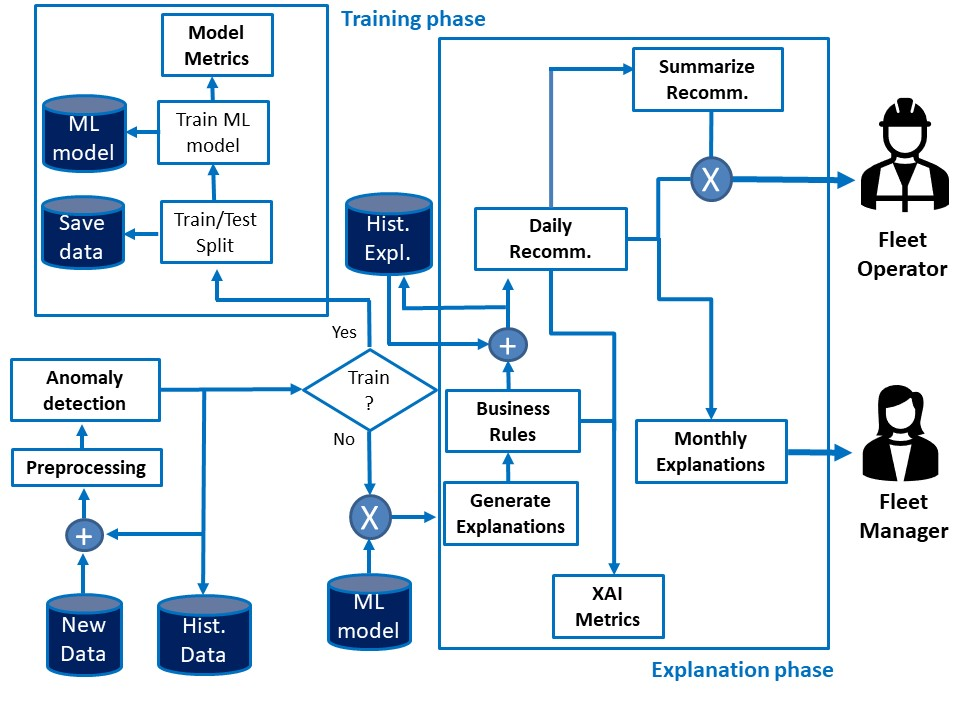
\includegraphics[width=320pt]{figures/chapter6_LucaFleet/FlowchartFinal.jpg}
  \end{tabular} 
  \caption{General flowchart followed by the fuel RecSys, as described in \hyperref[subsec:ch6-process-overview]{Subsection} \ref{subsec:ch6-process-overview}}
  \label{fig:ch6-flowchart-fuel-recsys}
\end{figure*}

Then, the process either applies the training phase for creating a new ML model, or applies the explanation phase, using one previously trained. 
For the training phase, the process trains an interpretable ML model \hyperref[subsec:ch6-ml-model]{Subsection} \ref{subsec:ch6-ml-model} and obtains its metrics in terms of model performance \hyperref[subsec:ch6-model-metrics]{Subsection} \ref{subsec:ch6-model-metrics}.

For the explanation phase, the process loads the ML model already trained, and uses it for generating explanations over the new data. They are combined with business rules in order to assure a minimum explanation quality \hyperref[subsec:ch6-business-rules]{Subsection} \ref{subsec:ch6-business-rules}. The explanations are stored and combined with previously generated ones. Then, they are used for generating daily recommendations that show the potential fuel that could be saved for each vehicle \hyperref[subsec:ch6-daily-recommendations]{Subsection} \ref{subsec:ch6-daily-recommendations}. The explanation phase also includes XAI metrics that can be used both for comparing the explanations generated by different models, as well as for measuring their quality by themselves \hyperref[subsec:ch6-xai-metrics]{Subsection} \ref{subsec:ch6-xai-metrics}.

Finally, the fuel saving recommendations are adjusted considering the audience that will receive them. There are two types of audiences considered for this purpose; a) \textbf{fleet operators} that receive the information about individual vehicles that have anomalous fuel consumption, together with recommendations that can be applied for reducing it; b) \textbf{fleet managers} that receive general explanations about the impact of driving behaviour features in the fuel consumption of the whole fleet, as well as information about the fuel consumption of vehicle models without taking into consideration the extra amount caused by the inefficient driving style \hyperref[subsec:ch6-recomm-user-profiles]{Subsection} \ref{subsec:ch6-recomm-user-profiles}. \hyperref[fig:ch6-ExplanationsDashboardExample]{Figure} \ref{fig:ch6-ExplanationsDashboardExample} shows an example of the final output explanations for those two user profiles. 

\begin{figure*}
\centering
  \begin{tabular}{c@{\qquad}c@{\qquad}c}
  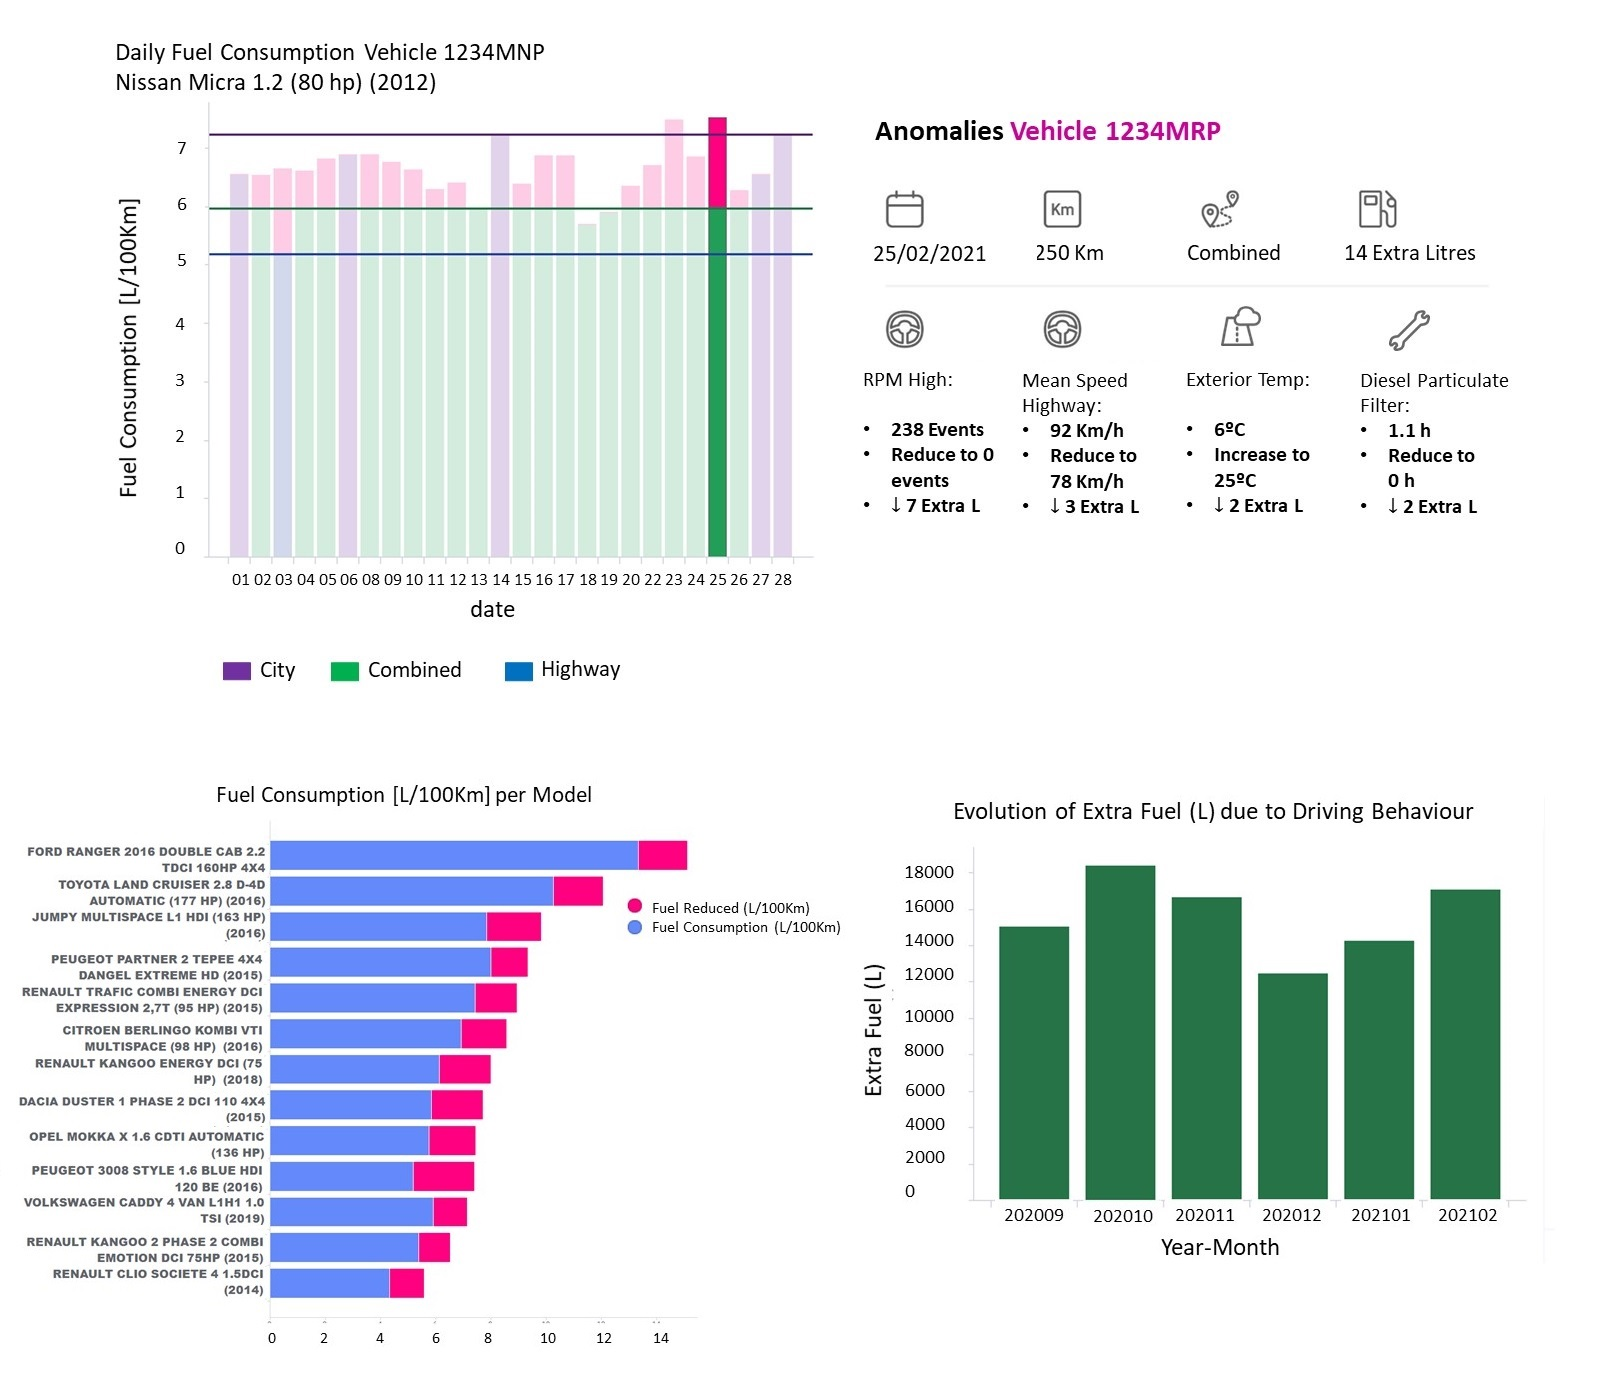
\includegraphics[width=0.9\columnwidth]{figures/chapter6_LucaFleet/ExplanationsDashboardExample.jpg}
  \end{tabular} 
  \caption{Example of explanations and recommendations for Fleet Operators (above) and Fleet Managers (below).\label{fig:ch6-ExplanationsDashboardExample}}
\end{figure*}

\subsection{Data preprocessing}\label{subsec:ch6-data-processing}
First, we obtain the daily aggregated information for each of the vehicles within the fleet through the telematics devices connected to the OBD-II (On-Board Diagnostics) on each of them. This generates real-time information of the vehicle's status. A sample of these raw data with a csv structure can be seen in \hyperref[table:ch6-sample-structure]{Table} \ref{table:ch6-sample-structure}.

\begin{table}[h!]
\centering
\resizebox{350pt}{!}{%
\begin{tabular}{llll}
\textbf{time\_tx} & \textbf{vehicle\_id} & \textbf{variable\_id} & \textbf{variable\_value} \\ \hline
2020-10-31 00:02:34.073000+00:00 & b123 & EngineSpeed  & 1200 \\
2020-10-31 00:12:34.073000+00:00 & b124 & VehicleSpeed & 55   \\
2020-10-31 01:12:34.073000+00:00 & b125 & EngineSpeed  & 1200 \\
2020-10-31 02:02:34.073000+00:00 & b124 & TripFuel     & 3.1 
\end{tabular}
}
\caption{Sample of the received data from the telematics devices}
\label{table:ch6-sample-structure}
\end{table}

We are interested in a daily vision of the vehicle for providing recommendations for the user profiles with a daily granularity level. Thus, we aggregate the raw information into a set of features, described at \hyperref[sec:annex-fuel-features]{Section} \ref{sec:annex-fuel-features} in the \hyperref[ch:annex]{Annex}. The features chosen correspond to a domain prior knowledge, since they must be related to vehicle's fuel consumption \parencite{zacharof2016review}. These features appear within the literature as potential causes of increased fuel usage both from the driving behaviour influence in fuel economy \parencite{zhang2017safedrive}, as well as from the vehicle status and exterior conditions \parencite{zhou2016review}. These features have already been proven useful for predicting fuel consumption with ML models \parencite{9072728, 8727915, perrotta2017application, barbado2021understanding}.

The features are divided into 4 groups: Index, Categorical, Explainable and Target. They are described below (though, for more detail, we refer to \hyperref[sec:annex-fuel-features]{Section} \ref{sec:annex-fuel-features} in the \hyperref[ch:annex]{Annex} \ref{ch:annex}).

\begin{itemize}
    \item \emph{Index features} refer to features used to identify each row (namely a vehicle's unique id, and the date).
    \item \emph{Categorical features} refer to non-numerical features used to distinguish group of vehicles, such as "vehicle model", which indicates vehicles with the same make-model, or "route type" for identifying the primary route type on a specific date (highway, city or combined). 
    \item Regarding the \emph{Explainable Features}, they are further divided into six groups. First, there are features related to the vehicle status itself. For instance, the pressure of the tires. If the pressure is too low, the fuel needed to cover the same amount of distance will increase, thus increasing the fuel consumption of the vehicle. These features are identified as \emph{vehicle condition}. 
    The next group of features are the \emph{Driving Behaviour} ones. They correspond to features related to the vehicle's driver behaviour itself that may affect the fuel consumption. An example of these features is the idle time spent. More idle time may increase fuel consumption.
    Another group of features considered are the \emph{Weather Variables}. For instance, the exterior temperature may affect a vehicle's thermodynamic cycle, harming its efficiency. Related to that, there is another group of features, called \emph{Road Conditions} for addressing the driving context (e.g. the time driving in a road with bumps). The final two groups are features related to the \emph{Operational Mass} of the vehicle, and to the extra fuel consumption from the usage of \emph{Auxiliary Systems} (e.g. time with air conditioning on). 
    \item The final feature is the \emph{target} column, the fuel consumption itself. This is calculated directly as: 
    \begin{equation}
    fuel\;consumption\;(L/100Km) =  \frac{trip\;fuel\;used\; (L)}{trip\;distance\;(kms)} \times 100
    \end{equation}\myequations{Vehicle fuel consumption}
\end{itemize}

This yields a data frame where each row corresponds to the daily aggregated values of the selected features for a specific vehicle. 

\subsection{Unsupervised anomaly detection in vehicle fuel consumption}\label{subsec:ch6-anomaly-detection}
Using the previous FAR data frame, the next step detects the vehicle-dates where there is an anomalous fuel consumption. Since there is no prior knowledge on when the fuel consumption is anomalous, we need to detect it in an unsupervised manner. Also, the module needs to provide a threshold value to distinguish outliers from inliers, since we want to include that information as a visual explanation.

To comply with both requirements, we apply an univariate unsupervised anomaly detection approach using a Box-Plot that classifies data points as outliers if they are above or below a specific threshold. \hyperref[eq:ch6-boxplot-anomalies]{Equation} \ref{eq:ch6-boxplot-anomalies} shows these thresholds using a 1.5 multiplier, which corresponds to approximately $\pm2.7\sigma$ (where $\sigma$ is the standard deviation) and 99.3\% coverage of the data for a normal distribution \parencite{mcgill1978variations, krzywinski2014visualizing}. This approach, with the 1.5 standard multiplier, has already been used within other vehicle-related contexts for anomaly detection in the energy usage \parencite{yin2019voltage, schuster2015lithium}.

In our case, the Box-Plot is applied over the different combinations of the categorical variables (make-model with vehicle\_group and route type with route\_type), obtaining different limits depending on the combination considered. We use this approach since the fuel consumption of a vehicle will change depending on the route type (e.g. city vs highway) and depending on the vehicle model \parencite{rakha2011virginia, zacharof2016review}.

\begin{equation}\label{eq:ch6-boxplot-anomalies}
\begin{split}
lim\_sup = Q3 + 1.5 \times IQR \\
lim\_inf = Q1 - 1.5 \times IQR
\end{split}
\end{equation}\myequations{Boxplot limits for anomaly detection in vehicle fuel consumption}

\subsection{ML model for generating for connecting input features and fuel consumption}\label{subsec:ch6-ml-model}
The following step is the training of a ML supervised model that finds relationships between the explainable and categorical features from the FAR data set and the target variable. Within this step, we could use any whitebox model that yields feature relevance-based global explanations. The main proposal is based on EBM \parencite{nori2019interpretml}, since its a whitebox algorithm with good predictive power that has been previously used within the fuel consumption context \parencite{barbado2021understanding}. With that, we have an interpretable model that can provide explanations about the relationship between input features and output fuel consumption, while being able to model complex non-linear relationships.

However, there are two problems that arise with EBM within the context of fuel consumption. First, the feature relevance explanations will be the same for all the vehicles within the fleet. That means that the unitary impact from, for instance, one extra speeding event, will be the same for passenger cars than for trucks if the fleet contains both types of vehicles. This could be fixed by using the pairwise terms of EBM to adjust each feature. For instance, $f_i(x_i) + f_ij(x_i, x_j)$ will be the adjusted feature relevance value for feature $x_i$ considering the vehicle model $x_j$. The problem is that we will need to adjust every combination of features and vehicle models, and this will significantly increase the number of features used for training the ML model. Our proposal for this problem is addressed with our EBM variation (EBM\_var) algorithm, which is detailed later.

Another problem is that the relationship between feature values and feature relevance may not be monotonic when it should be. For instance, more time driving in idle mode should always lead to more fuel consumption, and not to less. The original proposal of EBM does not allow for the usage of monotonic constraints. Because of that, we will also evaluate the usage of the CGA2M+ algorithm \parencite{watanabe2021cga2mplus}, where we can specify monotonic constraints. An example of these problems is shown in \hyperref[fig:ch6-ProblemsEBM]{Figure} \ref{fig:ch6-ProblemsEBM}.

\begin{figure}[h!]
\centering
  \begin{tabular}{c@{\qquad}c@{\qquad}c}
  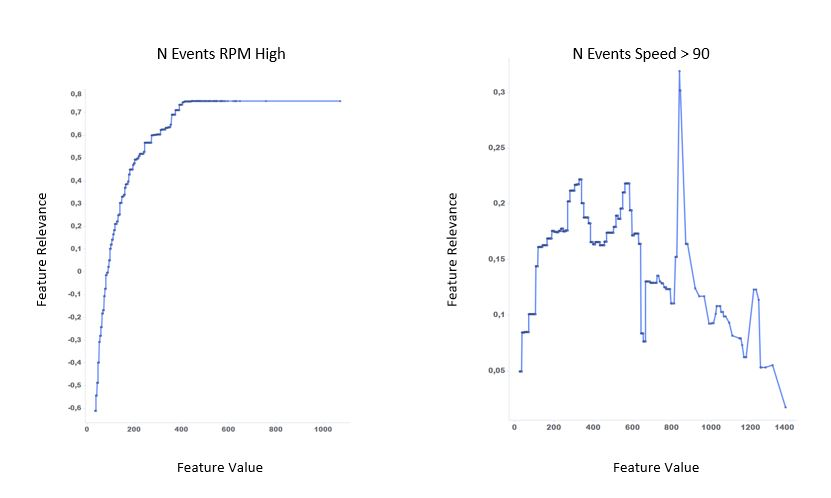
\includegraphics[width=300pt, height=180pt]{figures/chapter6_LucaFleet/ProblemsEBM.jpg}
  \end{tabular} 
  \caption{Problems with EBM. Left, we see that even though the evolution is monotonic by directly using EBM, the model uses one pairplot for every model in the fleet. Right, we see an example of a pairplot that should be monotonic but it is not.}
  \label{fig:ch6-ProblemsEBM}
\end{figure}

Our final solution will use the proposal that yield best results, according to the metrics defined at \hyperref[subsec:ch6-metrics]{Subsection} \ref{subsec:ch6-metrics}. % TODO, dejarlo así o hablar de que usamos EBM\_var?

\textbf{EBM variation}\label{subsec:ch6-ebm-var-intro}\\
The EBM variation that we propose considers possible differences that may exist within different subgroups of vehicles in order to adjust feature relevance and predictions. Regarding our use case, the feature relevance may be different depending on the vehicle group. For instance, the impact on the fuel consumption for each additional harsh brake may change depending on the vehicle's model and make considered. Thus, there should be different feature relevance-values pairs depending on that vehicle group category. Using only one EBM provides unique pairs of value-relevance regardless of the vehicle group, meaning that the final impact in the target variable will be the same for a specific feature value.

The intuition behind our proposal is similar to other works in the literature \parencite{waeto2017forecasting}. We add an additional layer of models to predict the error of a previous one. As represented in \hyperref[fig:ch6-ebm-variation-flowchart]{Figure} \ref{fig:ch6-ebm-variation-flowchart} for one subgroup of vehicles, first, we train an EBM model over all data during the training phase. Then, we predict the error for each of the vehicle's subgroups, and train additional EBM to predict that error and both improve the predictions of the first one as well as adjusting the results to the specificity of each of the subgroups. This last consideration is based on the fact that while the first model provides unique feature relevance-values pairs (because the second one is predicting the error of the first one in order to add it to its prediction), we can also use the feature relevance values of the second one to add them to the first one. This may be done since the feature relevance values of the second model show the feature contribution to the error.
With that, there will be different feature relevance-value pairs, as well as predictions, for each of the subgroups considered.

\begin{figure}[h!]
\centering
 \begin{tabular}{c@{\qquad}c@{\qquad}c}
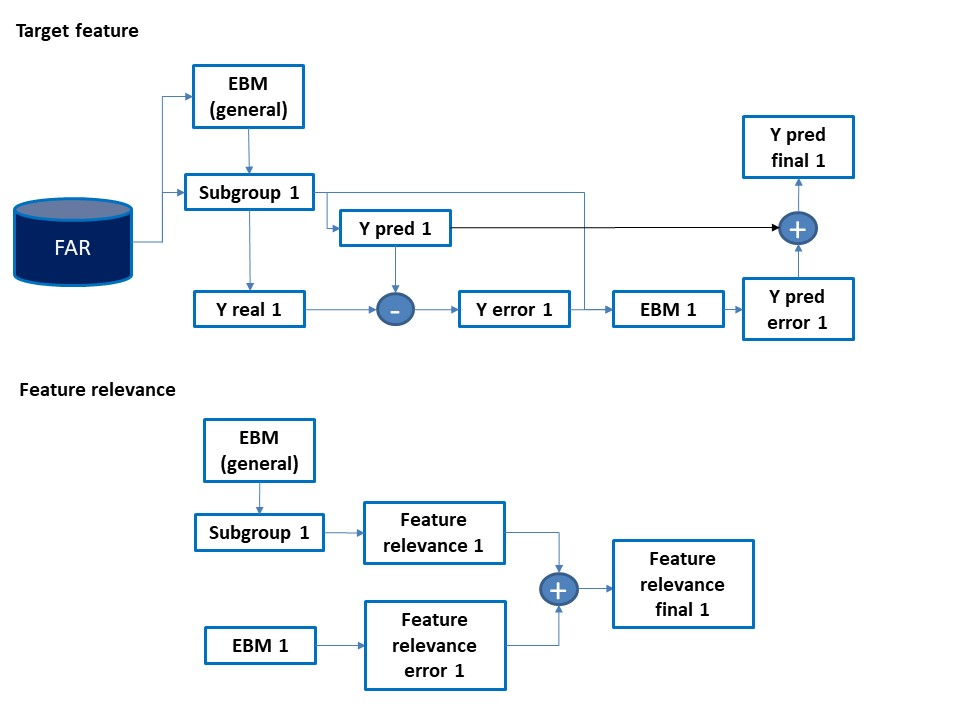
\includegraphics[width=280pt, height=200pt]{figures/chapter6_LucaFleet/EBM_variation.jpg}
  \end{tabular} 
  \caption{Proposal of the "EBM variation" over only one subgroup.  \label{fig:ch6-ebm-variation-flowchart}}
\end{figure}

The detailed description of EBM variation appears at \hyperref[subsec:annex-ebm-var]{Subsection} \ref{subsec:annex-ebm-var} in the \hyperref[ch:annex]{Annex}. 

\subsection{Generate explanations}\label{subsec:ch6-generate-explanations}
The "Generate explanations" step extracts the relationship between the fuel consumption of a vehicle in a specific date and the input features (FAR). This relationship is expressed in
\hyperref[eq:ch6-y-pred]{Equation} \ref{eq:ch6-y-pred}.

\begin{equation}\label{eq:ch6-y-pred}
y\_pred (n) = \varepsilon + \sum_{i=1}^{k}  f_{i}(x_{i}(n))
\end{equation}\myequations{Vehicle fuel consumption prediction based on the EBM output}

\hyperref[eq:ch6-y-pred]{Equation} \ref{eq:ch6-y-pred} shows the relationship for a data point \textit{n} between the predicted value of the target variable y\_pred with respect to \textit{k} input features, $x_{i}$, through their $f_{i}(x_{i}(n))$ functions. Thus, for a specific data point $n$ and feature value $x_{i}(n)$, we get the corresponding feature relevance $f_{i}$, obtaining the individual contribution of that feature in that data point to the predicted fuel consumption.
In all the cases, we train models without using pairwise terms, since they will potentially make the explanations and recommendations too complex. Thus, the explanations will not consider the joint evolution of two features (e.g., the joint evolution of a feature like 'mean exterior temperature' with 'hours raining', even though they may be related).

\subsection{Business rules}\label{subsec:ch6-business-rules}
Over the raw explanations, we apply the following business rules:
\begin{itemize}
\item \textbf{BR1}: The features used for training the model may be numeric (e.g. time driving uphill) or categorical (e.g. the vehicle model). All those categorical features are one-hot encoded before training the model. However, they are not considered for the explanations since they are not actionable (e.g., changing the vehicle model may lead to less fuel consumption under the same circumstances, but it is not something that can be acted upon easily in order to change it. Opposed to this are actionable features, like 'harsh brakes', which can be changed more easily from one day to another).
\item \textbf{BR2}: We remove the features in the vehicle-date explanations that have a very low impact on the fuel consumption (relative impact below 1\%)
\item \textbf{BR3}: The explanations only include vehicles where the average fuel consumption is above the value of the median inlier vehicles for the same model and on the same route type.
\item \textbf{BR4}: Feature values must be higher than the median value of the vehicle inliers from the same model for that same feature when the feature Type is Positive, or lower when Type is Negative.
\item \textbf{BR5}: The total fuel reduction from the explanations should not be more than the 80\% of the original fuel consumption\footnote{The value of 80\% is decided based on \hyperref[table:ch2-sota-FeatureInfluenceReduced]{Table} \ref{table:ch2-sota-FeatureInfluenceReduced} and \parencite{zacharof2016review}: considering the mean fuel reduction per category, using the upper limit values, we get a potential maximum reduction of 89.1\%. Since considering all the features together with their maximum contribution is an extreme case, we have validated with domain experts to set it to 80\%}. Since the models do not allow to impose restrictions in the learning for the individual models for the features, we need to apply this post-hoc filtering to remove explanations that are not physically possible.
\end{itemize}
EBM and EBM\_var do not necessarily yield monotonic explanations for each feature. Because of that, in this step we include an optional monotonicity filter in order to filter some of the feature relevance - feature values combinations from among all vehicles, and leave only those that result in a monotonic relationship between them. This filtering is optional, and can be used both for selecting only some particular explanations, or for computing a monotonicity metric that measures the degree of monotonicity for each feature in the data set \hyperref[subsec:ch6-xai-metrics]{Subsection} \ref{subsec:ch6-xai-metrics}. 

The \textbf{Monotonicity filter} analyses each pair of feature value and feature relevance for every vehicle group and route type combination and discards the pairs that are not monotonic. An example can be seen in \hyperref[fig:ch6-monotonicity-filter-example]{Figure} \ref{fig:ch6-monotonicity-filter-example}.
Starting from the evolution of the relevance-value pair of a particular feature, in this step the process finds the feature values intervals where the feature relevance is not monotonic, and discards those combinations. Thus, the raw explanations for each vehicle-day, where all the features are included, are filtered so that the feature values that correspond to feature relevance ones that are not monotonic are not included. 
\hyperref[fig:ch6-monotonicity-filter-example]{Figure} \ref{fig:ch6-monotonicity-filter-example} shows the original feature relevance-value pairs for a combination of route type and vehicle group for the feature count\_harsh\_brakes. As the figure shows, the evolution is not monotonic. It also shows the final result after applying the monotonicity filter.

\begin{figure}[h!]
\centering
 \begin{tabular}{c@{\qquad}c@{\qquad}c}
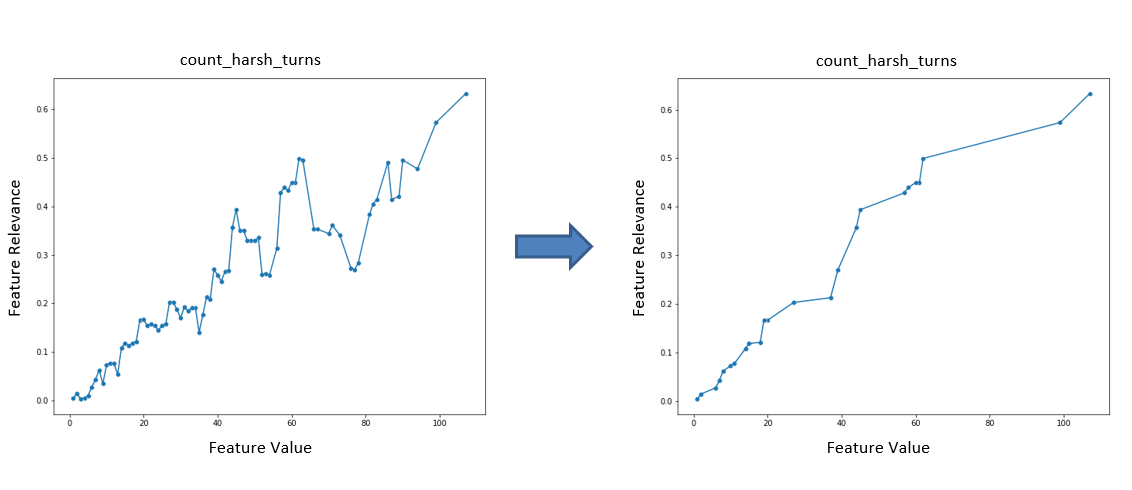
\includegraphics[width=350pt]{figures/chapter6_LucaFleet/MonotonicFilterExample.PNG}
  \end{tabular} 
  \caption{Example of evolution of the feature value and the feature relevance for feature count\_harsh\_brakes before and after applying the monotonicity filter\label{fig:ch6-monotonicity-filter-example}}
\end{figure}

A detailed description of the algorithm appears within the \hyperref[subsec:annex-monotonicity]{Subsection} \ref{subsec:annex-monotonicity} in the \hyperref[ch:annex]{Annex}. Since the monotonicity filter analyses the combined evolution of both feature relevance and feature value, it works either for EBM (where there is only one value-importance pair per feature at the dependency function \parencite{nori2019interpretml}), EBM\_var (where there is potentially one value-importance pair per feature and vehicle group), as well as with other XAI algorithms such as LIME and SHAP (where there may be more than one importance value per unique feature value \parencite{molnar2019interpretable}). Indeed, there may be more than one importance-value pair per feature value. However, since \hyperref[subsec:annex-monotonicity]{Subsection} \ref{subsec:annex-monotonicity} checks a pair and the immediate following one, it will, for instance, check $(x0,y0)$ against $(x0, y1)$ with $y1 > y0$, and will remove the latter if the importance is lower.

This approach is known as \textit{Informed Explainability} within the taxonomy of \parencite{beckh2021explainable}, since we are applying the prior knowledge not over the underlying blackbox model (the anomaly detection algorithm in this case), but over the XAI method itself. In particular, our approach works with \textit{formalized priors for explanations} since the knowledge is elicited through the literature, instead of using other approaches such as human-on-the-loop.

\subsection{Daily recommendations}\label{subsec:ch6-daily-recommendations}
Whitebox models that include feature relevance are useful for counterfactual explanations \parencite{arrieta2020explainable}. Since there is a unique intercept and unique feature relevance-value pairs, they can provide counterfactual explanations where one of the feature values alone may be changed, recalculating the predicted target value to see how it will change. These counterfactual explanations can be used as recommendations since they show future scenarios when particular actions take place.

The intuition behind it is the following one. "Generate Recom." changes the feature values of the outliers used within the explanation phase to a reference value (e.g. the corresponding median feature value of the inliers belonging to the same vehicle group and route type). This is applied for one feature at a time and for every feature labeled as "actionable" \footnote{As already mentioned, changing a feature like the vehicle model may lead to less fuel consumption under the same circumstances, but it is not something that can be acted upon easily in order to change it. Opposed to this are actionable features, like 'harsh brakes' or 'jackrabbits', which can be changed more easily from one day to another. These features were decided with the input received from domain experts}. Then, by subtracting the relative change in the predicted value from the real fuel consumption, it indicates which vehicles-dates would have a fuel consumption below the outlier limit for that vehicle group and route type. 

The details are described in \hyperref[alg:ch6-get-recom]{Algorithm} \ref{alg:ch6-get-recom}; getRecom function receives the historical median values of the inliers (obtained during the training phase; $X_{med}$), the data points of the explanation phase with their feature relevance ($X_{exp}$), and two lists, one with the explainable features that are actionable ($l_a$) and one with the categorical ones ($l_c$). It also receives a list $l_z$ with the features that are going to be explained using a zero value reference (for instance, by reducing the "harsh brakes" to zero, instead of the median value for that vehicle group). Using these inputs, getRecom function initializes two empty lists ($l\_up\_ind$ and $l\_up\_all$) and gets the feature relevance for the median inliers feature values ("coeff"), or zero value, with $checkPairwise(X_{med}, l_c, l_z)$ function. 
After obtaining the feature relevance, the function analyses every data point ($x$) within the explanations and obtains its predicted target value ($y\_pred$) using the feature relevance and the intercept. It also stores the real value ($y\_real$) of the target feature. Then, it checks every feature ($f$) within the explanations and gets its corresponding feature relevance from the median inliers reference, or the zero value reference, ($\beta_{fn}$). Then, it sums again all the feature relevance and intercept for data point x, without the feature relevance for feature "f". This leads to a new predicted value ($y\_new$) where all the other feature values are kept the same, but but with a change on the specific feature considered. The difference between $y\_pred$ and $y\_new$ is $\Delta$, and this difference is used to compute the change in the real fuel consumption ($l\_up\_ind$). After iterating for all the available combinations, getRecom uses groupVal function to obtain the estimated value in case all the actionable features change at the same time to their references (either zero or their median inlier value). This is done by aggregating all the individual changes in the prediction for each feature and subtracting the aggregated difference from the real fuel consumption.

% Recommendations
\begin{algorithm}[h!]
\caption{Generate Recommendations}\label{alg:ch6-get-recom}
\begin{algorithmic}[1]
\Procedure{getRecom}{$X_{med}, X_{exp}, l_a, l_c, l_z$}
    \State $l\_up\_ind \gets null$
    \State $l\_up\_all \gets null$
    \State $coeff \gets checkPairwise(X_{med}, l_c, l_z)$
    \For{$x \in X_{exp}$}
        %\State $y\_pred \gets \varepsilon + \sum_{i=1}^{k}  \beta_{i}(x_{i}) \times x_{i} $
        \State $y\_pred \gets \varepsilon + \sum_{i=1}^{k}  F_{i}(x_{i}) $
        \State $y\_real \gets x[target]$
        \State $comb \gets x[l_c]$
        \For{$f \in l_a$}
            \State $\beta_{fn} \gets coeff[f]$
            %\State $y\_new \gets \varepsilon + \sum_{i=1}^{k \neq f}  \beta_{i}(x_{i}) \times x_{i} $
            \State $y\_new \gets \varepsilon + \sum_{i=1}^{k \neq f}  F_{i}(x_{i})$
            %\State $y\_new \gets y\_new + \beta_{fn} \times X_{med}[comb]$
            \State $y\_new \gets y\_new + \beta_{fn}$
            \State $\Delta \gets y\_pred - y\_new$
            \State $y\_updated \gets y\_real - \Delta$
            \State $l\_up\_ind \gets l\_up\_ind.append(y\_updated)$
        \EndFor
    \EndFor
    \State $l\_up\_group \gets groupVal(l\_up\_ind, l_a, X_{exp}, l_c)$
    \State \textbf{return} $l\_up\_ind, l\_up\_group$
\EndProcedure
\end{algorithmic}
\end{algorithm}

Thus, \hyperref[alg:ch6-get-recom]{Algorithm} \ref{alg:ch6-get-recom} provides a list with the new estimated fuel consumption value for every individual feature change and for every vehicle-date pair ($l\_up\_ind$). Comparing these values against the outlier limit for that vehicle group and route type, we can see which individual feature changes will turn outliers into inliers, and what would be the new fuel consumption. It also provides a similar result but considering that every actionable feature changes at the same time ($l\_up\_group$). 

% TODO: Puedo meter aqui la tabla de ejemplo de salida del "Understanding..."

\subsection{Recommendations according to user profiles}\label{subsec:ch6-recomm-user-profiles}
According to \parencite{arrieta2020explainable}, explanations should be tailored for the specific profile of the user that will receive them, taking into account both their expectations and their domain knowledge. Within the use case proposed in this chapter, we identify two user's profiles: fleet operators and fleet managers.

\textbf{Fleet operators} are responsible for the status of the vehicles. Their main interest in explanations is detecting what vehicles are consuming excessively, and what is causing it, considering for that not every feature, but only the ones that are actionable, according to \hyperref[sec:annex-fuel-features]{Section} \ref{sec:annex-fuel-features} in the \hyperref[ch:annex]{Annex}. To accomplish that, the recommendations generated at \hyperref[subsec:ch6-daily-recommendations]{Subsection} \ref{subsec:ch6-daily-recommendations} may be enough. However, providing information for every combination of dates, vehicles and route types in terms of the numeric feature relevance may be overwhelming, not being useful for them. Therefore, we provide the recommendations for these users at two different levels. First, a summary of the main recommendations for a specific period of time (e.g. a month), where we only show vehicles that have a recurrent behaviour that impacts in the fuel consumption (e.g. always with driving behaviour related features). Second, we provide the individual daily detail only if they want to dive deeper into a particular vehicle and route type. In both cases, we only include vehicles with fuel consumption anomalies.

For the other profile, \textbf{fleet managers}, the main interest is having a global comparative view at a vehicle model level, not seeing information about individual vehicles or specific dates. Explanations should be expressed in terms of extra litres of fuel consumed, because that can be immediately turned into an economic cost, as well as in terms of environmental impact. For this profile, it is also useful not to consider all types of features in the explanations, but only the ones related to driving behaviour, since they are among the features with more impact \parencite{zacharof2016review}, they are actionable, and they are mainly associated to inefficient driving styles.
With that, after having the individual recommendations from \hyperref[alg:ch6-get-recom]{Algorithm} \ref{alg:ch6-get-recom}, the individual explanations are aggregated for the whole fleet and for each vehicle model, considering only for the potential fuel reduction features related to driving behaviour. A final comment is that these explanations include all data points, not only the outliers since it is an aggregated view.

\subsection{Metrics}\label{subsec:ch6-metrics}
There are two aspects to measure through metrics: model performance and quality of the explanations/recommendations. For the first case, we measure the predictive power of the surrogate ML model by seeing how close the predictions to the real fuel consumption value of the different vehicle-dates are. We will further refer to them as \textit{model metrics}. 

The second group of metrics are the ones obtained during the explanation phase, which are used for assessing several quality aspects within both the explanations and the final fuel saving recommendations. These metrics are useful for analysing the explanations by themselves, as well as for comparing the explanations generated between every model. We will further refer to them as \textit{XAI metrics}. Even though it may be difficult (or not reliable) to compare individual explanations from different models with certain metrics due to Rashomon's Effect \parencite{molnar2019interpretable}, the metrics that we propose analyze the explanations from a general perspective.

\subsubsection{Model performance metrics}\label{subsec:ch6-model-metrics}
\leavevmode\newline
Model metrics include metrics used for comparing the models among themselves. Here we use a test set to evaluate the model performance metrics. For that, we use we use the Adjusted R2 value (adj-R2) and the Mean Average Percentage Error (MAPE). We use adjusted R2 and MAPE, since they both yield a result in terms of percentage that can be easily understood.

All the model metrics are evaluated over a test set that includes both outliers and inliers, since the purpose is to measure how close the target feature predictions are to the real value. There are other potential metrics that can be considered, especially classification metrics that measure if after applying the anomaly limits over the predicted values, the inlier/outlier predicted class matches the one of the real target feature. However, since we are not using the ML surrogate model to actually predict the outlier/inlier class, we did not use them. 

\subsubsection{XAI metrics for assessing explanation quality}\label{subsec:ch6-xai-metrics}
\leavevmode\newline
Using the taxonomy of metrics in \parencite{carvalho2019machine} for individual explanations, we consider different properties for comparing the explanations generated by the different methods studied in this chapter. The properties considered are \textit{representativeness}, \textit{precision}, \textit{stability}, \textit{contrastiveness} and \textit{consistency with apriori beliefs} (as discussed in \hyperref[sec:ch2-metrics-xai]{Section} \ref{sec:ch2-metrics-xai}), since they address the main aspects of our use case. For stability and precision, we use metrics based on already existing metrics within the literature. For representativeness, contrastiveness and consistency with apriori beliefs, we propose additional ones that are useful for benchmarking the models within our use case. 
These metrics are used for evaluating the final explanations provided by the system (after applying all the business rules mentioned in the previous subsections unless otherwise indicated), and they are evaluated for anomalous vehicle-dates only. A summary of these metrics appear in \hyperref[table:ch6-xai-resume-metrics]{Table} \ref{table:ch6-xai-resume-metrics}.

\textbf{Representativeness} metrics measure the relevance or importance of the explanation. They include these metrics:
\begin{itemize}
    \item \textbf{n\_features}: Number of features used for fuel explanations for a particular vehicle-date. The metric appears in \hyperref[eq:ch6-xai-metrics-n-features]{Equation} \ref{eq:ch6-xai-metrics-n-features}, where $v$ is one vehicle, $t$ one date, $X^{'}(v,t)$ the remaining features after applying the business rules, and $card$ the cardinality.
    \item \textbf{rel\_importance}: Percentage of fuel covered by the features used in the explanations. The metric appears in \hyperref[eq:ch6-xai-metrics-rel-imp]{Equation} \ref{eq:ch6-xai-metrics-rel-imp}, with $f_{i}$ the dependency function for feature $i$, $\beta_0$ the intercept, and  $\beta_i$ the feature coefficient.
\end{itemize}

\begin{equation}\label{eq:ch6-xai-metrics-n-features}
\begin{aligned}
n\_features_{v,t} = card(X^{'}(v,t))
\end{aligned}
\end{equation}

\begin{equation}\label{eq:ch6-xai-metrics-rel-imp}
\begin{aligned}
rel\_importance_{v,t} = \frac{\beta_0 + \sum_{i=0}^{n\_features_{v,t}} {\beta_i \times f_{i}(x_{v,t})}} {y\_r(v,t)}
\end{aligned}
\end{equation}

\textbf{Precision} metrics measure how close is the fuel prediction to the real fuel value using the features within the explanations. For that, we use the MAPE (mean average percentage error) obtained by comparing that fuel prediction based on the final explanations against the real fuel consumption value. The metric appears in \hyperref[eq:ch6-xai-metrics-xai-mape]{Equation} \ref{eq:ch6-xai-metrics-xai-mape}, where $N_t$ are the number of data points for that vehicle $v$, $y\_p^{'}(v, t)$ the fuel prediction using the features remaining after the business rules, and $y\_r(v,t)$ the real fuel value for that vehicle and date.

\begin{equation}\label{eq:ch6-xai-metrics-xai-mape}
\begin{aligned}
xai\_mape_{v} =  \frac{\sum_{t=0}^{N_t} {mape(y\_p^{'}(v, t), y\_r(v,t))} } {N_t}
\end{aligned}
\end{equation}

\textbf{Stability} metrics include one metric, \textit{stability\_error}. This metric is based on the proposal of \parencite{melis2018towards}, as indicated in \hyperref[eq:ch6-stability-metric-sample]{Equation} \ref{eq:ch6-stability-metric-sample} within \hyperref[sec:ch2-metrics-xai]{Section} \ref{sec:ch2-metrics-xai}. For this particular metric, we do not filter the explanations using the business rules.

\begin{equation}\label{eq:ch6-stability_metric_sample}
\qquad 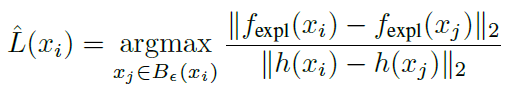
\includegraphics[width=200pt]{figures/stability_metric.PNG}
\end{equation}

\textbf{Contrastiveness} metrics measure the impact of the recommendations generated over the explanations provided by the XAI technique. These metrics are:
\begin{itemize}
    \item \textbf{per\_var}: Percentage of fuel saved for a particular vehicle-date after applying the recommendations provided by the system. It appears at \hyperref[eq:ch6-xai-metrics-per-var]{Equation} \ref{eq:ch6-xai-metrics-per-var}, where the numerator is the output from \hyperref[alg:ch6-get-recom]{Algorithm} \ref{alg:ch6-get-recom} for a vehicle $v$ and a date $t$ represented through $x(v,t)$, and the denominator $y\_r(v,t)$ is the real fuel value for that vehicle and date.
    \item \textbf{per\_below}: Percentage of anomalous vehicle-dates, within each vehicle model, that receive fuel recommendations that would change their fuel value below the anomaly threshold value.
\end{itemize}

\begin{equation}\label{eq:ch6-xai-metrics-per-var}
\begin{aligned}
per\_var_{v,t} = \frac{getRecom({X_{med}, x(v,t), l_a, l_c, l_z})[0][0]} {y\_r(v,t)}
\end{aligned}
\end{equation}\myequations{XAI metrics: contrastiveness}

\textbf{Consistent with Apriori Beliefs} metrics measure how aligned are the explanations with prior domain knowledge. It includes the following metrics:
\begin{itemize}
    \item \textbf{per\_mon}: Percentage of data points for a particular feature and model that are monotonic after applying the monotonicity filter, described in \hyperref[alg:annex-monotonicty]{Algorithm} \ref{alg:annex-monotonicty} in the \hyperref[ch:annex]{Annex}. The details for this metric are within that subsection, at
    \hyperref[eq:annex-xai-metrics-mono]{Equation} \ref{eq:annex-xai-metrics-mono}.
    \item \textbf{MAPE vs reference fuel}: This metric computes the MAPE value of the new average fuel consumption (after the recommendations) against the catalog fuel reference for that model. 
    \item \textbf{\% below catalog}: It shows the percentage of vehicle-dates that are receiving a recommendation that turns the average fuel consumption (L/100Km) below the catalog reference (with an offset of 1 L/100Km). It should be minimized, because the target fuel should not be below the catalog reference (a value that is not physically reachable). 
\end{itemize}


\begin{table}[h!]
\centering
\resizebox{180pt}{!}{%
\begin{tabular}{@{}lll@{}}
\toprule
\textbf{Taxonomy}  & \textbf{Metric}       \\ \midrule
Representativeness & n\_features           \\
Representativeness & rel\_importance  \\
Precision          & xai\_mape             \\
Stability          & stability\_error      \\
Contrastiveness    & per\_var              \\
Contrastiveness    & per\_below            \\
Apriori Beliefs    & per\_mon     \\
Apriori Beliefs    & mape vs reference fuel     \\
Apriori Beliefs    & per\_below\_catalog     \\
\bottomrule
\end{tabular}%
}
\caption{Summary of the XAI metrics analysed, linking them to their taxonomy.}
\label{table:ch6-xai-resume-metrics}
\end{table}


\section{Evaluation}\label{sec:ch6-evaluation}
In this section, we indicate some aspects regarding the evaluations carried out. First, we describe the data sets that we have used in \hyperref[subsec:ch6-DataFleet]{Subsection} \ref{subsec:ch6-DataFleet} and the models configuration \hyperref[subsec:ch6-model-params]{Subsection} \ref{subsec:ch6-model-params}. Then, we focus on the evaluations themselves along with the hypothesis checked in \hyperref[subsec:ch6-eval-model-performance]{Subsection} \ref{subsec:ch6-eval-model-performance} for the evaluations regarding model performance, and in \hyperref[subsec:ch6-eval-xai]{Subsection} \ref{subsec:ch6-eval-xai} and \hyperref[subsec:ch6-eval-xai-apriori]{Subsection} \ref{subsec:ch6-eval-xai-apriori} for the XAI evaluations.

Our aim is to use this analysis for evaluating \textbf{H2} and \textbf{H1}, described in \hyperref[chap:3-objetives]{Chapter} \ref{chap:3-objetives} at
\hyperref[sec:Hypotheses]{Section} \ref{sec:Hypotheses}, within the context of vehicle fuel consumption, using our XAI proposal, which can be based on any of the three interpretable models described in \hyperref[sec:ch6-method]{Section} \ref{sec:ch6-method} (EBM, EBM\_var and CGA2M2+).

For checking \textbf{H1}, we evaluate our proposal through the XAI-specific metrics described in \hyperref[subsec:ch6-xai-metrics]{Subsection} \ref{subsec:ch6-xai-metrics}, in order to see if we can measure the quality of the explanations that indicate what features are causing that the vehicle fuel consumption is anomalous. Here, we benchmark the interpretable models alternatives in order to see if the explanations are significantly different.

Regarding \textbf{H2}, the use-case of vehicle fuel consumption is useful since there is extensive literature regarding the prior domain knowledge about what variables impact on the vehicle fuel consumption. For the evaluations of H2, we consider our proposal based on the "EBM\_var" interpretable model unless otherwise said. We analyse the following aspects:
\begin{itemize}
\item We first evaluate if there are significant differences in terms of model performance between our proposed EBM\_var and the original EBM. (\hyperref[subsec:ch6-eval-model-performance]{Subsection} \ref{subsec:ch6-eval-model-performance})
\item After that, we analyse if the model performance metrics for the three intepretable methods (EBM, EBM\_var and CGA2M2+) can be considered good enough on absolute terms. (\hyperref[subsec:ch6-eval-model-performance]{Subsection} \ref{subsec:ch6-eval-model-performance})
\item Then, we evaluate our XAI proposal, which takes into account prior domain knowledge, in order to see if the explanations generated for explaining the features that impact on the vehicles with anomalous fuel consumption are indeed aligned to that prior knowledge (\hyperref[subsec:ch6-eval-xai-apriori]{Subsection} \ref{subsec:ch6-eval-xai-apriori})
\item We also check if there are significant differences in XAI-specific metrics regarding other aspects besides prior domain knowledge. (\hyperref[subsec:ch6-eval-xai]{Subsection} \ref{subsec:ch6-eval-xai})
\item Finally, we analyse if our proposal yields similar results in terms of model performance compared to SOTA blackbox models. Thus, we see if there is a trade-off or not between an interpetable model that includes domain knowledge against a blackbox model that aims to optimize only model performance within this context. (\hyperref[subsec:ch6-eval-model-performance]{Subsection} \ref{subsec:ch6-eval-model-performance})
\end{itemize}

We will carry out an study with EBM and EBM\_var that both considers the usage of the monotonicity filter for adjusting the final explanations or not. The first analysis will not use this filtering for two reasons. First, because it is a filter that is only applicable to EBM and EBM\_var, and we want to perform a comparison against CGA2M2+ that uses the same business rules in all three cases. Second, because it will just dampen the impact of the explanations. Thus, in order to see if EBM\_var is aligned with prior domain knowledge, first we are going to see the least conservative case (with the explanations without the filter), knowing that if the full explanations are aligned with prior knowledge, since the filtered ones are a subset of them, they should also be aligned. Nonetheless, we will include a XAI metric comparison considering the explanations after the monotonicity filter.

With that, the analyses on this chapter provide a full evaluation of the sub-hypotheses described in this thesis, thus answering the main hypothesis. The reason behind it is that we evaluate the quality of explanations through XAI metrics after using domain knowledge for generating them, we  check if the explanations are aligned to that domain knowledge, and we see if there is a significant penalty on model performance or not by enforcing the explanations to follow that prior knowledge.

\subsection{Data involved}\label{subsec:ch6-DataFleet}
We consider 9 data sets, belonging to different fleets, as shown in \hyperref[table:ch6-data-description]{Table} \ref{table:ch6-data-description}. These data sets are samples for some of their vehicles, and the aggregated information includes information collected during 2019, 2020 and 2021. The table indicates the data set (Fleet), the number of individual vehicles (Vehicles), the number of vehicle groups (Models), the unique combinations of vehicle-dates (Points), the N points that are associated with an anomalous fuel consumption according to the proposal of \hyperref[sec:ch6-method]{Section} \ref{sec:ch6-method} (Outliers), and how many of those data points are within the test set (Outliers [test]). Together with that, we also include a fleet size category (Fleet Size) following the one that appears in \parencite{fleet2021trends}, where fleets with more than 500 vehicles are considered "enterprise) (or large), fleets between 50 and 499 "medium", and fleets with less than 49 vehicles "small". All the vehicles have either petrol or diesel engines.

\begin{table}[h!]
\centering
\resizebox{280pt}{!}{%
\begin{tabular}{@{}lllllll@{}}
\toprule
\textbf{Fleet} &
  \textbf{Vehicles} &
  \thead{\textbf{Fleet} \\ \textbf{Size}}&
  \textbf{Models} &
  \textbf{Points} &
  \textbf{Outliers} &
  \thead{\textbf{Outliers} \\ \textbf{[test]}}
  \\ \midrule
D1 & 1552 & Large & 16 & 219707 & 5772  & 577    \\
D2 & 1568 & Large & 16 & 121160 & 1809  & 181    \\
D3 & 316  & Medium & 44 & 65549  & 10484 & 1046   \\
D4 & 252  & Medium & 14 & 35394  & 1944  & 193    \\
D5 & 165  & Medium & 20 & 22478  & 724   & 71     \\
D6 & 143  & Medium & 20 & 18635  & 2003  & 201    \\
D7 & 33   & Small & 5  & 9733   & 949   & 95     \\
D8 & 20   & Small & 5  & 2235   & 349   & 35     \\
D9 & 3    & Small & 2  & 300    & 10    & 2      \\ \bottomrule
\end{tabular}%
}
\caption{Data set description, including the number of data points, number and type of vehicles.}
\label{table:ch6-data-description}
\end{table}

We train a model over each one of those data sets, using the 90\% of the data points for training, and the remaining 10\% for testing. As already mentioned, the model's performance metrics are analyzed considering all the test data points (comparing the model's prediction of the average fuel consumption versus the real value). For the XAI metrics used for assessing the explanations generated (the ones that appear within the explanations and recommendations from the method in \hyperref[sec:ch6-method]{Section} \ref{sec:ch6-method}), as well as for the study of explanation alignment with prior domain knowledge, we either use the whole outlier set, or we use the outlier data points that are within the test set (depending on the metric). This last aspect is indicated within every specific metric analysis.

\subsection{Model configuration}\label{subsec:ch6-model-params}
The hyperparameters used for every model match the default ones provided by the software libraries used (only modifying the parameters related to the monotonic constraints regarding CGA2M+). The reason behind that is that we ran several experiments with different hyperparameter configurations, but we did not found significant improvements from a statistical point of view in model's performance metrics when compared to the results using the default hyperparameters.  Regarding "EBM variation", both the EBM and EBM\_var use the same hyperparameter configuration.

\subsection{Model performance evaluation}\label{subsec:ch6-eval-model-performance}
In this subsection, we include the evaluations regarding the model performance. They are studied 
considering both outliers and inliers, and using the raw model predictions (without the business rules).

\subsubsection{Comparison between EBM, EBM\_var and blackbox models}\label{subsubsec:ch6-comparison-vs-blackbox}
First, we address the comparison between the different models using several model performance metrics in order to see if there are significant differences between the predictive power of the ML models analysed in this chapter. For that, we perform a k-fold cross-validation (CV) over the train data set using 30 splits. For every one of those splits, we train a model on a subset of the training data and evaluate it over the validation data selected by k-fold CV. This is done for each of those 30 splits, and for one data set per each fleet size (choosing the one with more data points) in order to have a representative analysis over different types of data sets. Thus, we consider D1, D3 and D7. 

This yields a vector of 30 components for each data set-metric-ML model that will be used for comparing against the other combinations of ML models belonging to the same data set-metric. The comparison is carried out by using Wilcoxon signed-rank test \parencite{wilcoxon1992individual} in order to see if the metrics of two of the ML models are similar. Wilcoxon signed-rank test is chosen for this hypothesis testing since it's a non-parametric test that can be applied over paired or potentially related data. This last consideration is important since the metrics obtained after the k-fold CV may be related to some degree, because the same data sets are used for different models, and the metrics from a k-fold of a particular data set-metric-ML model may be using similar training data compared to another k-fold.

Thus, we check the p-value resulting from the hypothesis test in order to see if H0 is rejected (H0 = distributions are equal), using 0.05 as the threshold value for rejecting H0.

The results of the evaluation appear in \hyperref[table:annex-model-metrics-contrast]{Table} \ref{table:annex-model-metrics-contrast} within \hyperref[subsec:ch6-annex-fleet-results-performance-contrast]{Subsection} \ref{subsec:ch6-annex-fleet-results-performance-contrast}. That table contain the pair of models compared ("model\_1" and "model\_2"), along with the metric considered and the median value  for the 30 k-fold splits used at every data set (for example,  D\_7\_m\_2 is the median value for model\_2 with the metric considered at data set 7). It also includes the p-value from Wilcoxon signed-rank test at each data set (P1 is the p-value at D1, and so on). 

First, we analyse the \textbf{comparisons regarding a baseline model, ElasticNet} (labeled as "linear\_model"). Out of all the metrics and data sets, \textbf{in 93\% of the cases there are significant differences between this model and the other ones}, while this model has a worst median value (higher error metrics, lower r2 and explained variance). This highlights how the predictive power of ElasticNet for our use case is almost always significantly worse than using any of the other models considered.

The next analysis that we consider is regarding XGBoost results versus LightGBM. The expected result is that their metrics should be similar, as reported in different benchmarks within the literature \parencite{nemeth2019comparison}, \parencite{anghel2018benchmarking}. Out of the 18 combinations of metrics-data sets, 13 of them (72\%) have significantly different metrics distributions according to the hypothesis test. Regarding D1 and D3, in all the metrics the results from XGBoost outperform those from LightGBM (lower error metrics, higher r2 and explained variance) considering those cases with p-values$<$0.05. However, for the cases with p-values $<$ 0.05 in D3, LightGBM offer better results. The gap between the metrics, however, is clearly smaller than the one comparing ElasticNet (p.e. the median value r2 for D3 is 0.65 for XGBoost, 0.675 for LightGBM, while being 0.28 for ElasticNet). 

Regarding the comparisons between LightGBM and EBM, we see that 11 out of the 18 data sets-metrics combinations (61\%) have significantly different metric distributions. In all those cases, EBM are worse than those from LightGBM (higher error metrics, lower r2 and explained variance), though with a much smaller difference than that compared to ElasticNet (p.e. for instance, the median r2 value for D1 is 0.67 for EBM and 0.69 for LightGBM).

Something similar happens when comparing XGBoost versus EBM. There are no significant differences regarding D7, but the differences regarding D1 and D3 are bigger since XGBoost obtained better metrics than LightGBM for those data sets. The percentage of data sets-metrics that have significantly different distributions comparing EBM to XGBoost is also 11 out of 18 (61\%).

These analyses show how EBM matches XGBoost for model performance over D7. However, there are significant differences between those two models in all the metrics of data sets D2 and D1, even though the difference between them is much lower than the one compared to ElasticNet (EBM significantly outperforms ElasticNet in 17 out of 18 data set-metric combinations).
Also, it matches LightGBM metrics regarding the "median\_absolute\_error" in all data sets, as well as the "max\_error" in D3 and D7, and the r2 score and explained variance at D3. 

The next step is comparing the results from EBM\_var. \textbf{Comparing against the base EBM, EBM\_var outperforms it in 7 out of the 18 data set-model combinations}. The cases where it outperforms EBM all belong to D1 and D3, the data sets with more registers. This happens due to the fact that D7 have many vehicle\_groups where the number of registers do not meet the threshold th\_ebm\_var, hence the model used is the base EBM and that lead to the exactly the same metrics. So, the proper comparison is regarding D1 and D3 only. Thus, it outperforms the base model in 7 out of the 12 data set-model combinations. This includes all the metrics except for "max\_error" in both data sets, and "mean\_squared\_error" in D3.

Comparing EBM\_var to LightGBM, we see how the 11 different combinations from EBM change significantly. In these comparison, there are only 3 (16.7\%) metric distributions ("median\_absolute\_error" for D1 and D3, and "mean\_absolute\_error" for D1), where EBM\_var actually outperforms LightGBM (lower error metric values).

Regarding XGBoost, there are only 2 significantly different metric distributions, belonging to the "median\_absolute\_error" at both D1 and D3. In those cases, EBM\_var also outperforms XGBoost.

With all these analyses, we first see regarding EBM, that even though its metrics are significantly lower than those form XGBoost and LightGBM, it only takes place for some combinations of data sets-metrics. And even then, the differences are significantly lower than those against the baseline model ElasticNet. 
Second, we see how using \textbf{EBM\_var significantly improves the results, offering a model that generally matches in performance both XGBoost and LightGBM, even outperforming them for some data sets and metrics combinations}.

To visually illustrate these comparisons, we include with \hyperref[fig:ch6-model-metrics-mean-squared-error]{Figure} \ref{fig:ch6-model-metrics-mean-squared-error} the model metrics results for mean squared error as an example.

\begin{figure}[h!]
\centering
 \begin{tabular}{c@{\qquad}c@{\qquad}c}
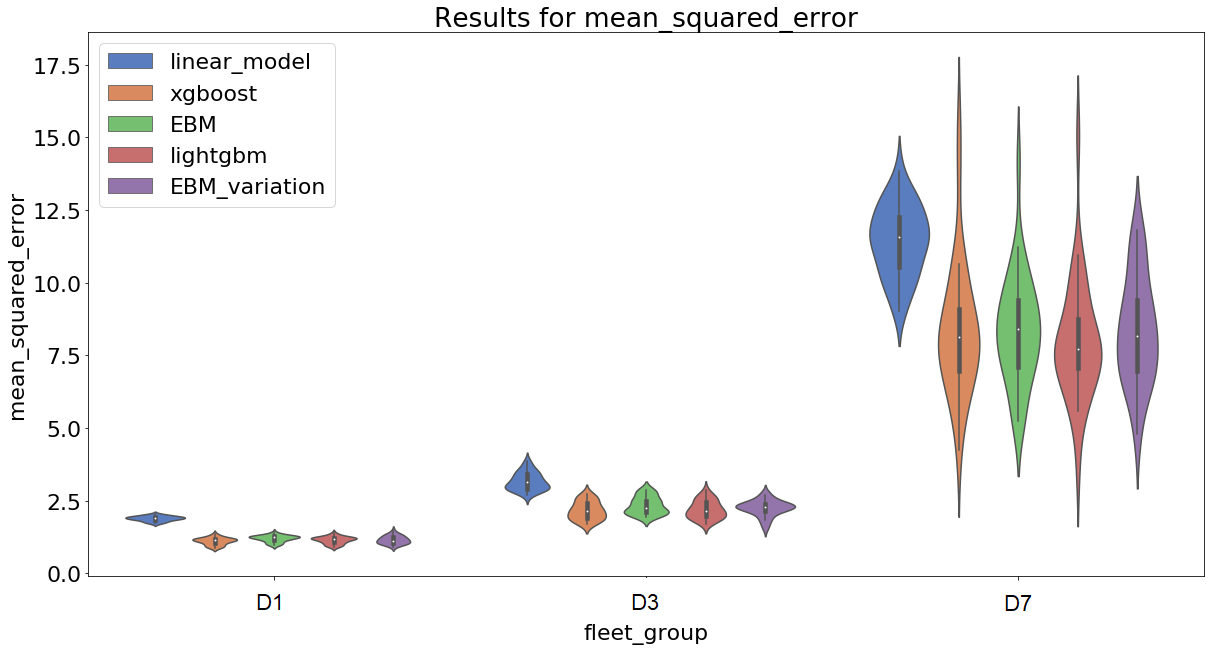
\includegraphics[width=0.8\columnwidth]{figures/chapter6_LucaFleet/model_metrics_mean_squared_error.PNG}
  \end{tabular} 
  \caption{Model metric results for mean squared error. X-axis include the metric value, and Y-axis the three different data sets used.\label{fig:ch6-model-metrics-mean-squared-error}. It shows similar metrics regarding EBM and EBM\_var compared to XGBoost and LightGBM.}
\end{figure}

%\textbf{Analysis of the quality of the model performance metrics}\\
\subsubsection{Analysis of the quality of the model performance metrics}\label{subsubsec:ch6-quality-model-performance}
After the previous analysis, we check the results from \textbf{EBM, EBM\_var, and CGA2M+} over the different data sets in order to see if the results are good enough over the test set (all test set, not only outlier data), and using the raw model predictions (without the business rules).

Regarding adj-R2, even if it's clear that it indicates the proportion of the variance in the target feature that can be predicted using the input features, it is not trivial to define value thresholds to indicate if the model is good or not. It heavily depends on both the context and the units of the target feature \parencite{hair2016primer, hair2013partial}. However, there are some guidelines that may be considered. As a reference, we use the proposal of \parencite{chin1999structural} that mentions the following levels: $0.67$ \textit{substantial}, $0.33$ \textit{moderate} and $0.19$ \textit{weak}.

MAPE, is a metric commonly used for forecasting models. However, it can be also useful for regression tasks \parencite{de2016mean}. Though it is also not direct to define thresholds for MAPE, we use as reference the ones detailed in \parencite{lewis1982industrial}, originally proposed for forecasting models: $<0.1$ \textit{highly accurate}, $[0.1-0.2]$ \textit{good}, $[0.2-0.5]$ \textit{reasonable} and $>0.5$ \textit{inaccurate}.

The metrics over the test set for each ML model used for predicting the fuel consumption over each one of the data sets considered appear in \hyperref[table:ch6-mape-r2-test]{Table} \ref{table:ch6-mape-r2-test}, where we see the mean MAPE over each vehicle in every data set, as well as the adjusted R2 metric for all the predictions in every data set. \textbf{For EBM\_var, we  see that in all data sets the MAPE value is \textit{highly accurate}, with the exceptions of D3, D4 and D9) where is \textit{good}. The same happens with CGA2M+, with the exception of D4, which is \textit{highly accurate} in this case . For Adjusted R2, EBM\_var is always within the \textit{substantial} category, except for the case of D4, where it is \textit{moderate}. The same happens with CGA2M+.}

\begin{table}[h!]
\centering
\resizebox{280pt}{!}{%
\begin{tabular}{@{}llllllll@{}}
\toprule
\textbf{\begin{tabular}[c]{@{}l@{}}Data \\ set\end{tabular}} &
  \textbf{\begin{tabular}[c]{@{}l@{}}MAPE \\ EBM\end{tabular}} &
  \textbf{\begin{tabular}[c]{@{}l@{}}MAPE\\ EBM\_var\end{tabular}} &
  \textbf{\begin{tabular}[c]{@{}l@{}}MAPE\\ CGA2M+\end{tabular}} &
  \textbf{\begin{tabular}[c]{@{}l@{}}Adjst R2\\ EBM\end{tabular}} &
  \textbf{\begin{tabular}[c]{@{}l@{}}Adjst R2\\ EBM\_var\end{tabular}} &
  \textbf{\begin{tabular}[c]{@{}l@{}}Adjst R2\\ CGA2M+\end{tabular}} \\ \midrule
\textbf{D1} 
& \cellcolor{green!25}0.08 
& \cellcolor{green!25}0.08 
& \cellcolor{green!25}0.08 
& \cellcolor{green!25}0.77 
& \cellcolor{green!25}0.8  
& \cellcolor{green!25}0.79 \\
\textbf{D2} 
& \cellcolor{green!25}0.09 
& \cellcolor{green!25}0.08 
& \cellcolor{green!25}0.08 
& \cellcolor{yellow!25}0.66 
& \cellcolor{green!25}0.84 
& \cellcolor{green!25}0.85 \\
\textbf{D3} 
& \cellcolor{yellow!25}0.13 
& \cellcolor{yellow!25}0.11 
& \cellcolor{yellow!25}0.14 
& \cellcolor{green!25}0.94
& \cellcolor{green!25}0.96 
& \cellcolor{green!25}0.92 \\
\textbf{D4} 
& \cellcolor{green!25}0.09 
& \cellcolor{yellow!25}0.10 
& \cellcolor{green!25}0.09 
& \cellcolor{yellow!25}0.61 
& \cellcolor{yellow!25}0.64 
& \cellcolor{yellow!25}0.61 \\
\textbf{D5} 
& \cellcolor{green!25}0.09 
& \cellcolor{green!25}0.08 
& \cellcolor{green!25}0.08 
& \cellcolor{yellow!25}0.66 
& \cellcolor{green!25}0.72 
& \cellcolor{green!25}0.72 \\
\textbf{D6} 
& \cellcolor{green!25}0.09 
& \cellcolor{green!25}0.07 
& \cellcolor{green!25}0.08 
& \cellcolor{green!25}0.85 
& \cellcolor{green!25}0.9  
& \cellcolor{green!25}0.86 \\
\textbf{D7} 
& \cellcolor{green!25}0.08 
& \cellcolor{green!25}0.07 
& \cellcolor{green!25}0.09 
& \cellcolor{green!25}0.8  
& \cellcolor{green!25}0.83 
& \cellcolor{green!25}0.82 \\
\textbf{D8} 
& \cellcolor{green!25}0.08 
& \cellcolor{green!25}0.08 
& \cellcolor{green!25}0.06 
& \cellcolor{yellow!25}0.63 
& \cellcolor{green!25}0.69 
& \cellcolor{green!25}0.67 \\
\textbf{D9} 
& \cellcolor{yellow!25}0.15
& \cellcolor{yellow!25}0.15 
& \cellcolor{yellow!25}0.17 
& \cellcolor{green!25}0.85 
& \cellcolor{green!25}0.84 
& \cellcolor{green!25}0.81 \\ \bottomrule
\end{tabular}%
}
\caption{MAPE and Adjusted R2 over the test set for each ML model and for each data set. Green cells indicate metrics that are inside the best category, while yellow indicate second best.}
\label{table:ch6-mape-r2-test}
\end{table}

\subsection{Prior domain knowledge evaluation}\label{subsec:ch6-eval-xai-apriori}
Now, we focus on analysing whether our proposal (for the case of EBM\_var) yields explanations that are aligned to prior domain knowledge or not. Since this evaluation is carried out over the explanations, we only focus on the vehicles that have fuel consumption anomalies (in all of them, not only in the test set). We also focus on the 4 months of data where the winter period is included (in order to be able to assess the impact of the ambient temperature). Using the models, we get the explanations for each vehicle-date for that period of data, and we aggregate the median feature impact values per subcategory and per vehicle fleet. The median results regardless of the fleet appear in \hyperref[figure:ch6-BoxPlotVehicleFuelImpact]{Figure} \ref{figure:ch6-BoxPlotVehicleFuelImpact}, and the median results considering fleet and including the limits from the SOTA appear in \hyperref[figure:ch6-FeatureImpactperDataset]{Figure} \ref{figure:ch6-FeatureImpactperDataset}. For the analyses, we have considered only vehicles that have a median MAPE over the test set of "Good forecasting" or better unless otherwise indicated (following the criteria from previous subsection).

The categories that we study are "Auxilary Systems" (for all the features that imply an additional electrical energy consumption), "Driving Behaviour" (driver-related features), "Road Conditions", "Vehicle Conditions" and "Weather Conditions". Regarding "Vehicle Conditions", we have included additional variables within the "Other" subcategory with respect to \parencite{zacharof2016review} (e.g. the additional fuel consumption when the DEF level is low), so it does not match the ones covered in that review. Because of that, this subcategory will not be used for checking the hypotheses already mentioned. We do not consider "Rain" subcategory, since the review only provides one reference value.

\begin{figure}[h!]
\centering
 \begin{tabular}{c@{\qquad}c@{\qquad}c}
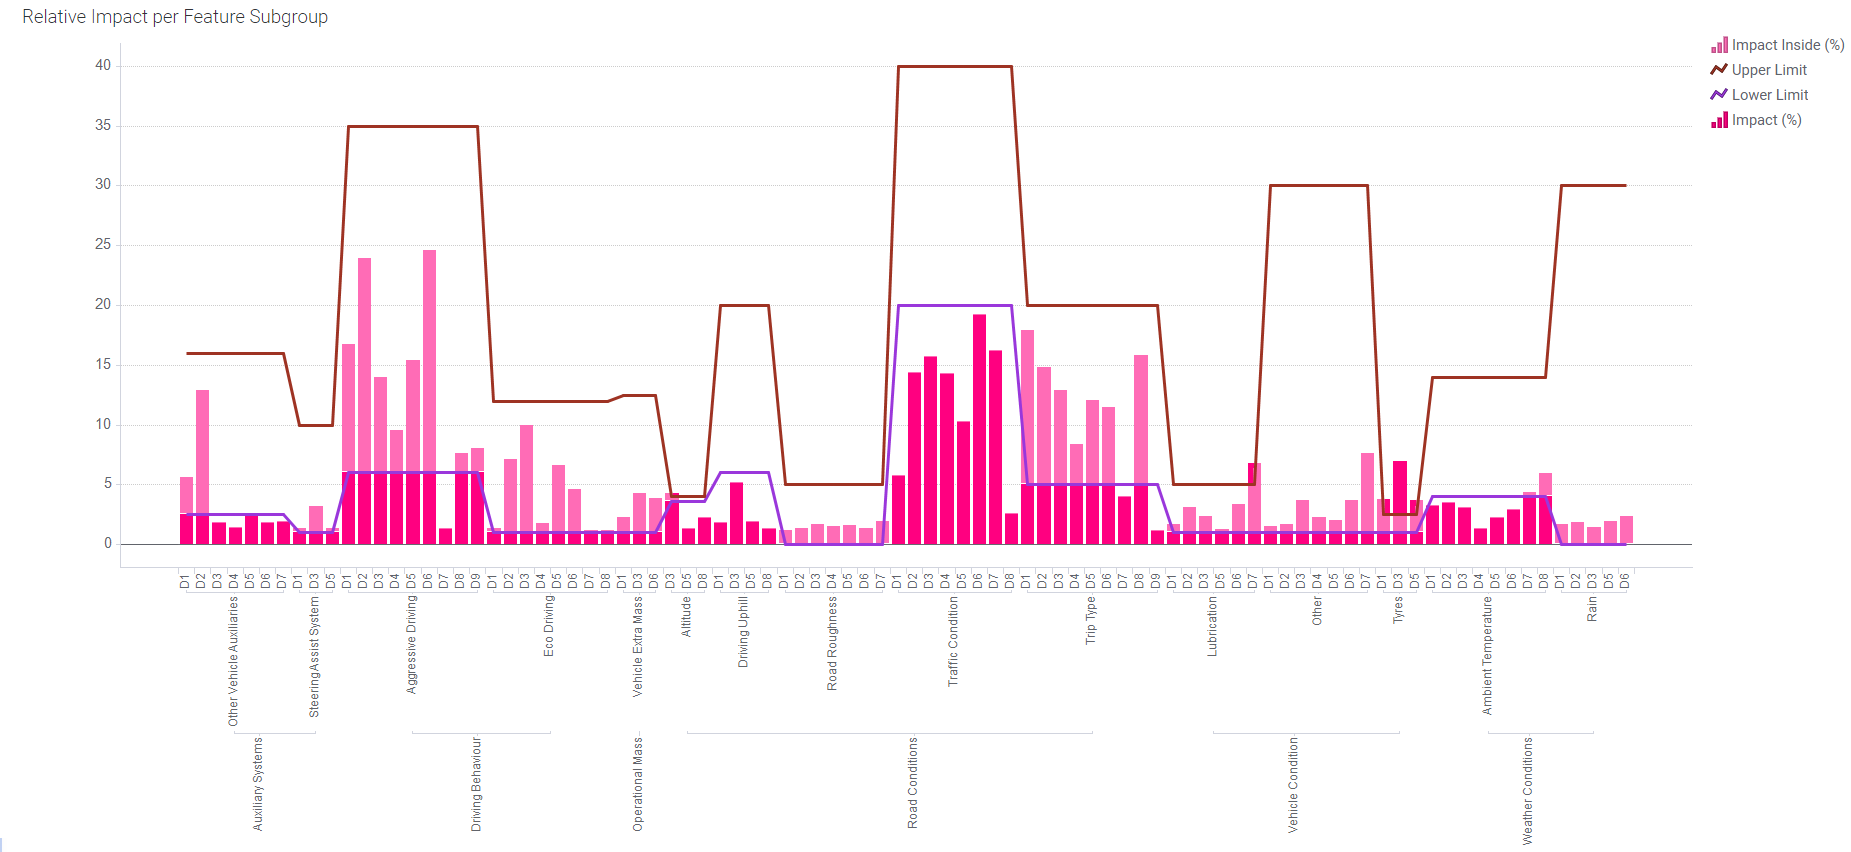
\includegraphics[width=0.95 \columnwidth]{figures/chapter6_LucaFleet/FeatureImpactperDataset.PNG}
  \end{tabular} 
  \caption{Median feature impact per Category-Subcategory-Fleet and the corresponding limits from the literature \parencite{zacharof2016review}  \label{figure:ch6-FeatureImpactperDataset}}
\end{figure}

Thus, in \hyperref[figure:ch6-FeatureImpactperDataset]{Figure} \ref{figure:ch6-FeatureImpactperDataset}, we see that, for 46 combinations, out of the 78 (without the Subcategories of "Other" and "Rain", as mentioned before), the feature relevance is within the limits from the SOTA. The remaining 32 that are not within the limits is because they are either lower than the minimum value used, or higher (for all the three data sets where tyres are relevant, and Lubrication for D7). "Aggressive Driving", "Eco-Driving", "Trip Type" and "Road Roughness" are the Subcategories that are both common in all data sets while having an aggregated feature impact that is within the literature limits. Others, such as "Steering Assist Systems" and "Vehicle Extra Mass" are also fully within the limits, but they are features that are relevant only for some data sets.

With \hyperref[figure:ch6-BoxPlotVehicleFuelImpact]{Figure} \ref{figure:ch6-BoxPlotVehicleFuelImpact} we see the individual impact per vehicle and date, for all the data sets considered together. As the figure shows, "Other Vehicle Auxiliaries", "Steering Assist Systems", "Aggressive Driving", "Eco Driving", "Vehicle Extra Mass", "Road Roughness", "Trip Type, and "Lubrication" have a median value per vehicle-date that is within the limits from the SOTA. For some Subcategories, such as "Steering Assist Systems", "Vehicle Extra Mass", and "Road Roughness", the upper whisker value from the boxplot is also within the SOTA limits. Other subgroups where the median value was not within the limit (because it was below the lower limit), the upper whisker is within the SOTA limits. This is the case of "Ambient Temperature", "Traffic Condition" and "Driving Uphill".
We see, however, that even though the impact per Subcategory normally does not exceed the upper values reported, there are data points where the impact is above the thresholds from the literature. 
%ch:sota
%table:sota-factors-table

\begin{figure}[h!]
\centering
 \begin{tabular}{c@{\qquad}c@{\qquad}c}
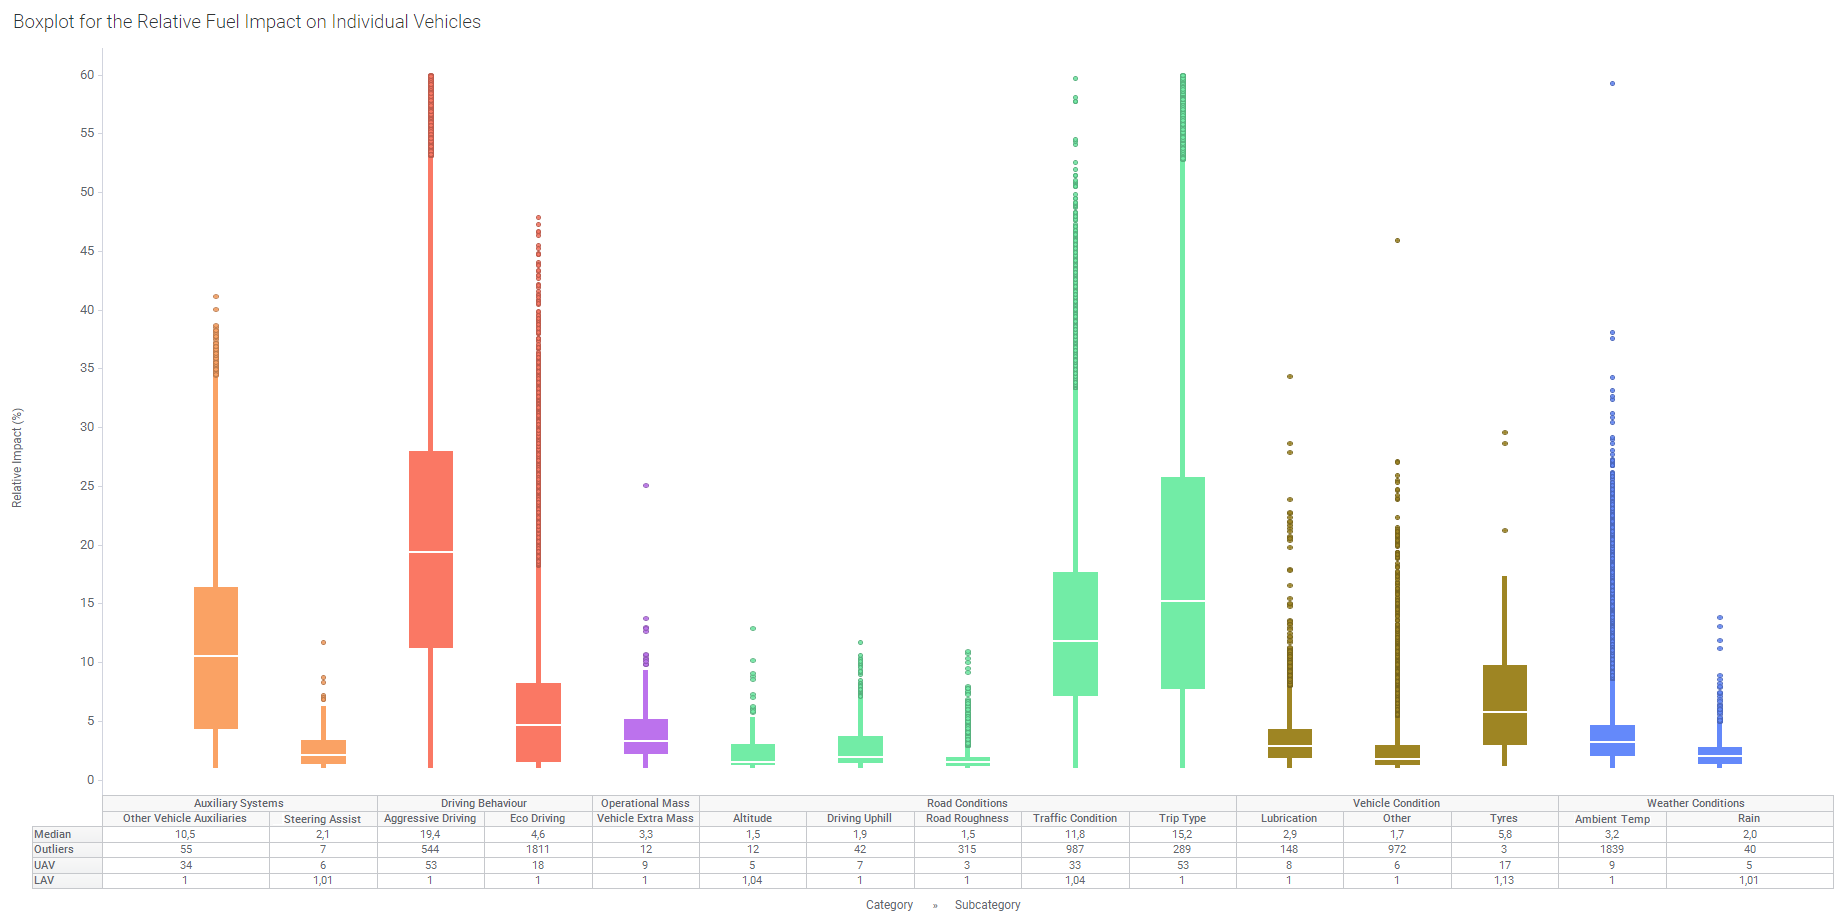
\includegraphics[width=0.9 \columnwidth]{figures/chapter6_LucaFleet/BoxPlotImpact.PNG}
  \end{tabular} 
  \captionsetup{justification=centering}
  \caption{Subcategory fuel impact per vehicle-date.\label{figure:ch6-BoxPlotVehicleFuelImpact}}
\end{figure}

With that, \textbf{we validate this analysis for the 74 out of the 78 combinations of subcategories-data sets since they have an influence in the fuel consumption because the relative impact is always below the maximum SOTA values, and in some cases, its even between them}. The exceptions are all the cases of the impact due to features associated to the "Tyres" subcategories, and "Lubrication" for D7.


\subsection{XAI evaluation}\label{subsec:ch6-eval-xai}
For this evaluation we assess the XAI metrics over the outlier explanations in terms of representativeness, precision, stability, contrastiveness and consistency with apriori beliefs, introduced in \hyperref[subsec:ch6-metrics]{Subsection} \ref{subsec:ch6-metrics}. For precision and stability, we use the outliers within the test set only, since they are metrics related to the prediction output itself. For the remaining XAI metrics, we use all the outlier data points.
The results are displayed in \hyperref[table:annex-xai-metrics-contrast]{Table} \ref{table:annex-xai-metrics-contrast}, showing the Kruskal-Wallis hypothesis contrast test \parencite{kruskal1952use} comparing the results between the three interpretable methods. The table shows the metric comparison in terms of the metric mean value, using the same date set-vehicle-date series when carrying out the comparison for a metric between two algorithms. The study is carried out over all the outlier data available (since we want to compare the explanation quality). We first compare the results without using the monotonicity filter (expect for obtaining \textit{per\_mon} metric), and then we compare the results using it.

Considering \textbf{representativeness} metrics, we analyse both the number of features used by the models within the explanations for a particular vehicle-date (\textit{n\_features}), and the percentage of fuel covered by the features used in the explanations (\textit{rel\_importance}). For all the combinations of algorithms-data set-metric we see statistically significant differences. Regarding \textit{n\_features}, we see that on Large and Medium data sets, EBM\_var is the algorithm that uses more features in the final explanations. However, for Small data sets, the one that uses more features is CGA2M+. This makes sense, since the benefits of EBM\_var only appear with a fleet that has a medium/large amount of vehicle models. For \textit{rel\_importance}, the results are also logical: it can be expected that \textit{rel\_importance} is higher in EBM than in EBM\_var since the former uses less features (meaning that EBM\_var is able to include more features, but that do not have a significant impact compared to the rest). 

For the \textbf{precision} XAI metric, we assess the predictive power of the explanations, which include the business rules for generating them, as opposed to the model's evaluation carried out before, which accounted only for the prediction itself, regardless of the explanations. On every type of data set, EBM and EBM\_var provide similar results. Compared to CGA2M+ the results are also similar, except for Medium data sets, where both EBM and EBM\_var outperform CGA2M+. We can also analyze the MAPE value of the metrics by themselves over the outliers and with the final explanations. Considering the MAPE thresholds defined previously, we see that on Large and Medium data sets, the predictive power with the final explanations and focusing only on the outliers (and only from the test set), is \textit{reasonable}, being very close to \textit{good} category. On Small data sets, the results are on the borderline between \textit{reasonable} and \textit{inaccurate}. This is related to the loss of predictive power due to the business rules constraints, as well as the relatively small data set considered (since we are only focusing on the outliers on the test set). Thus, even though the results are not necessary bad, what is interesting is that for some cases, the results are still accurate even after applying the business rules.

With \textbf{stability} metric, we do not see statistically significant differences in Large data sets. In Medium data sets, EBM is the algorithm with less stability error, while in Small data sets the best results are achieved by CGA2M+. With all that, we see that when there is enough data points, the stability error tends to be the same in all the models, and even though in those cases, generally EBM is the algorithm that achieves a lower stability error, having then the best results.

Regarding \textbf{contrastiveness}, there are many cases where the differences are statistically significant. In Large and Medium data sets, EBM\_var yields the best results in terms of percentage of fuel variation from the daily recommendations (\textit{per\_var}). In Small data sets, the best results are provided by CGA2M+. For the percentage of data points that will be below the anomaly threshold (\textit{per\_below}), we see similar results, with EBM\_var having the greatest reduction percentage for Large and Medium data sets, and CGA2M+ for Small ones. This is logical; when there are enough data points, the constraints on the explanations from the point of view of EBM\_var do not have a significant penalization, thus, the model is able to cover significant information with the explanations. However, for smaller data sets, imposing the constraints during the learning (CGA2M+) yields richer explanations.

In the case of \textbf{apriori beliefs}, we see the degree of monotonicity for EBM and EBM\_var, compared to the perfect degree of monotonicity from CGA2M+. We see that in both cases the degree of monotonicity is significantly lower than the perfect score, and that EBM is significantly more stable than EBM\_var in terms of this metric.

Thus, this first analysis, showed that \textbf{in Large and Medium data sets, the results from EBM\_var are solid, achieving good results on most of the metrics}. This indicates that when there are enough data points, the business rules and its associated constraints can be applied over this model, and still provide good results. The model is also able to use significantly more features and cover more fuel than either EBM or CGA2M+. \textbf{For Small data sets, the results are more contested}. It is true that EBM\_var is similar on several metrics to both EBM and CGA2M+, but \textbf{in some other cases, CGA2M+ provides better results}.

Continuing with the measurements of apriori beliefs, we check the MAPE value of the new average fuel consumption for each vehicle-date after from the final recommendations, \textbf{compared to the catalog fuel consumption} for the same make, model, year, fuel type and route type. For this analysis we only use D1, since it is the largest fleet and because we know exactly the vehicle models and its associated catalog fuel consumption reference. Results appear in \hyperref[table:ch6-comparison-fuel-reference]{Table} \ref{table:ch6-comparison-fuel-reference}, with MAPE 1 corresponding to the median MAPE versus the catalog fuel, MAPE 2 corresponds to the median MAPE versus the median fuel inlier vehicles, and MAPE 3 is the same as MAPE 2 but considering only explanations for outlier vehicles. The table also indicates the percentage of data points with a MAPE 1 below different threshold values (0.5, 0.2, 0.1). It also indicates the percentage of instances with a new fuel consumption below the catalog reference. We see that the results are similar for the three models, with CGA2M+ being better for the percentage of vehicles below the catalog fuel reference. 

\begin{table}[h!]
\centering
\resizebox{200pt}{!}{%
\begin{tabular}{@{}llllllll@{}}
  \textbf{Method} &
  \rot{\textbf{MAPE 1}} &
  \rot{\textbf{MAPE 2}} &
  \rot{\textbf{MAPE 3}} &
  \rot{\textbf{\% MAPE 1 \textless 0.5}} &
  \rot{\textbf{\% MAPE 1 \textless 0.2}} &
  \rot{\textbf{\% MAPE 1 \textless 0.1}} &
  \rot{\textbf{\% Below Catalog}} \\ \midrule
EBM      & 0.14 & 0.14 & 0.14 & 94.2 & 64.2 & 36.8 & 3.3 \\
EBM\_var & 0.15 & 0.14 & 0.14 & 93.2 & 62.6 & 35.6 & 3   \\
CGA2M+    & 0.14 & 0.13 & 0.14 & 94.4 & 63.9 & 36.7 & 2.6 \\ \bottomrule
\end{tabular}%
}
\caption{Different MAPE metrics for each of the models versus the catalog fuel consumption (MAPE 1), the median inliers (MAPE 2), or considering only the vehicles with outlier fuel consumption versus the inliers (MAPE 3).}
\label{table:ch6-comparison-fuel-reference}
\end{table}

\hyperref[fig:ch6-FuelReductionPerModel]{Figure} \ref{fig:ch6-FuelReductionPerModel} shows the average potential fuel reduction with each of the algorithms over every vehicle model and route type, considering the case of D1. We see how CGA2M+ generally provides fuel reductions that are more conservative than the other two methods. The advantage is that there are no cases where the new fuel consumption is below the catalog fuel reference. Comparing EBM\_var with EBM, we see that the first method generally provides recommendations that decrease more the fuel consumption.
This can be seen in \hyperref[fig:ch6-FuelImpactperFeature]{Figure} \ref{fig:ch6-FuelImpactperFeature} and \hyperref[fig:ch6-PairplotComparison]{Figure} \ref{fig:ch6-PairplotComparison}. In \hyperref[fig:ch6-FuelImpactperFeature]{Figure} \ref{fig:ch6-FuelImpactperFeature} we see the daily mean feature fuel impact (in L) for D1 comparing the different models. There, we see how some of the features that have a very high impact on fuel consumption for EBM and EBM\_var do not appear with CGA2M+ after retrieving the explanations and applying the business rules filters. This is the case of "rpm\_high". 

\begin{figure}
  \centering
  \begin{tabular}{c@{\qquad}c@{\qquad}c}
  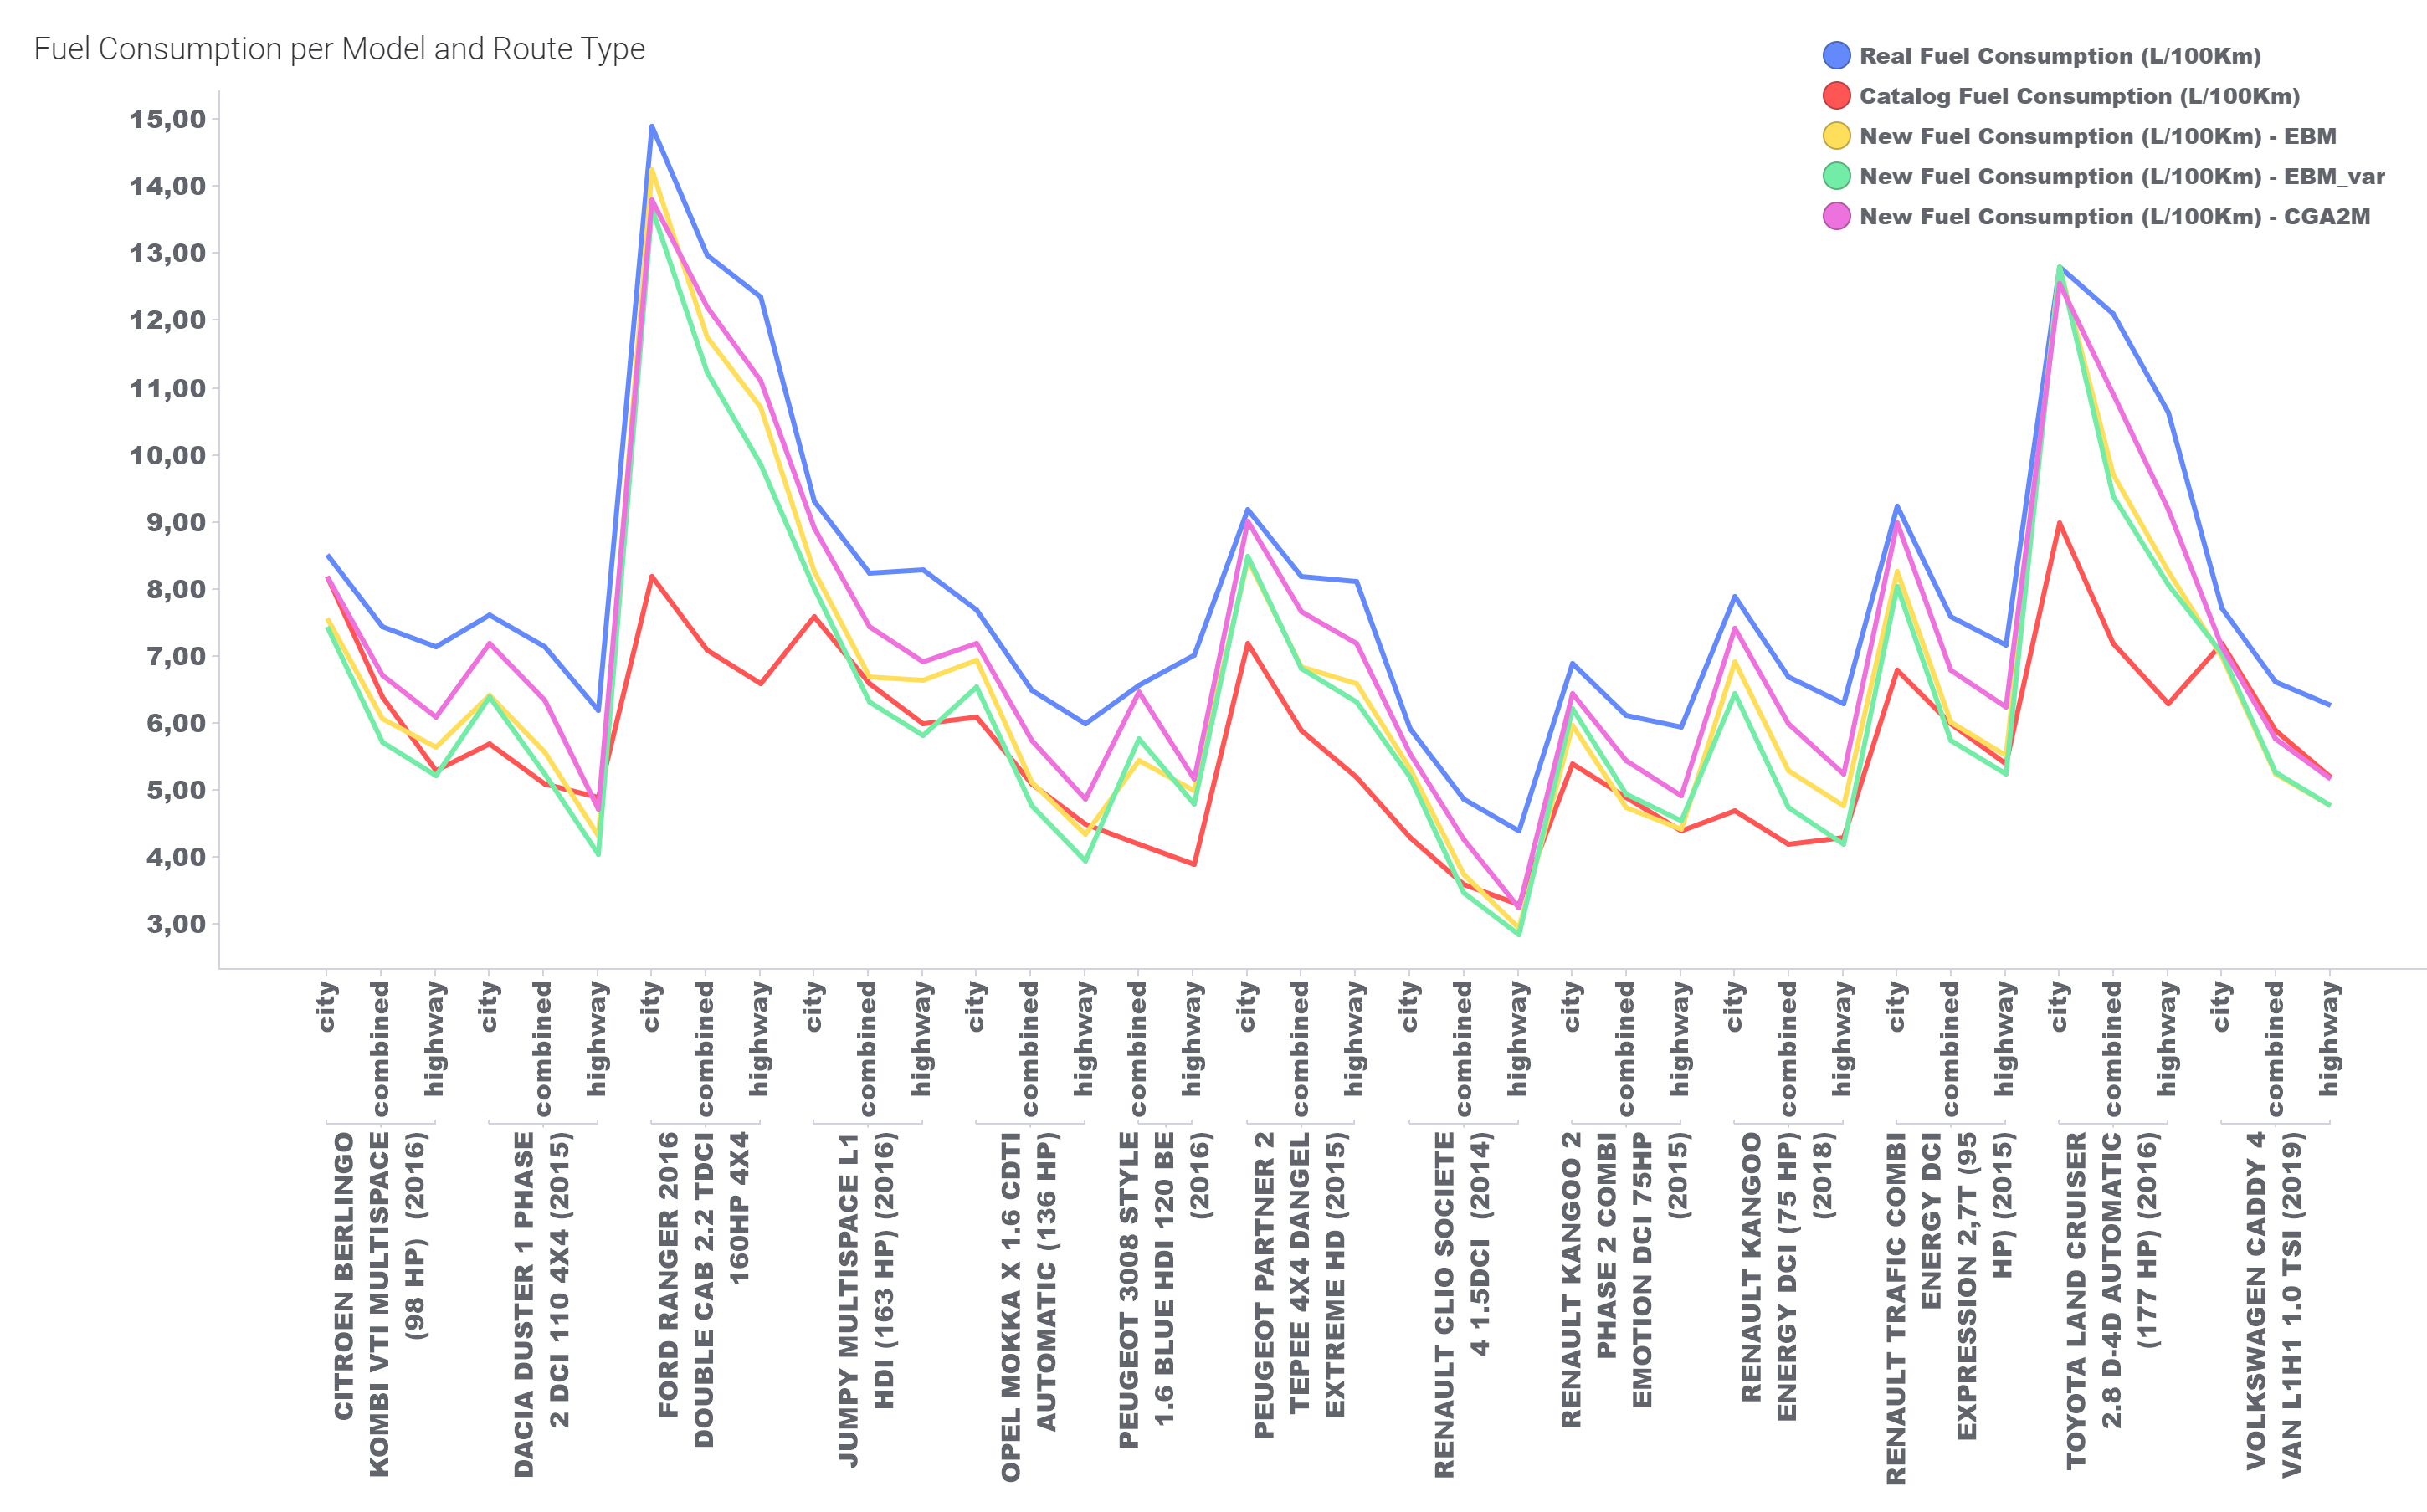
\includegraphics[width=420pt]{figures/chapter6_LucaFleet/FuelReductionPerModel.PNG}
  \end{tabular} 
  \caption{Comparison of the potential fuel reduction per vehicle model and route type for D1. The comparison includes the three algorithms with respect to both the real fuel consumption and the catalog reference.\label{fig:ch6-FuelReductionPerModel}}

  \begin{tabular}{c@{\qquad}c@{\qquad}c}
  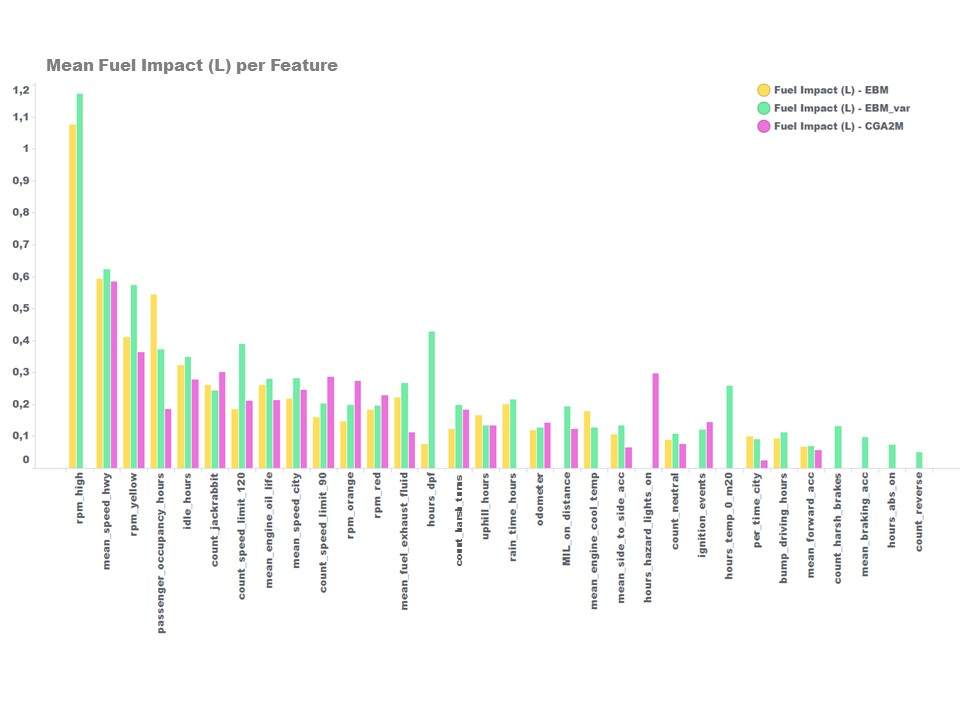
\includegraphics[width=410pt]{figures/chapter6_LucaFleet/FuelImpactperFeature.jpg}
  \end{tabular} 
  \caption{Daily mean feature fuel impact (in L) for D1, comparing the different models. Features shown appear at least within 100 vehicle-dates combinations.\label{fig:ch6-FuelImpactperFeature}}
\end{figure}

Focusing on some vehicle models and some of the features with higher impact, we see in \hyperref[fig:ch6-PairplotComparison]{Figure} \ref{fig:ch6-PairplotComparison} the relationship between feature relevance and feature values, using the data set D1. It shows how in many cases, the CGA2M+ curve is below the ones from the other methods, since it needs to be monotonic. We also see how EBM and EBM\_var are able to extract relationships that are almost monotonic (e.g. for "Trip Kms" or "Mean Speed Hwy"), while the relationships in other cases are clearly non monotonic (e.g. "Hours Raining" or "Count Events Speed $>$ 120 Km/h). This plot shows the values for EBM and EBM\_var before applying the monotonicity filtering.

\begin{figure*}
\centering
\begin{tabular}{c@{\qquad}c@{\qquad}c}
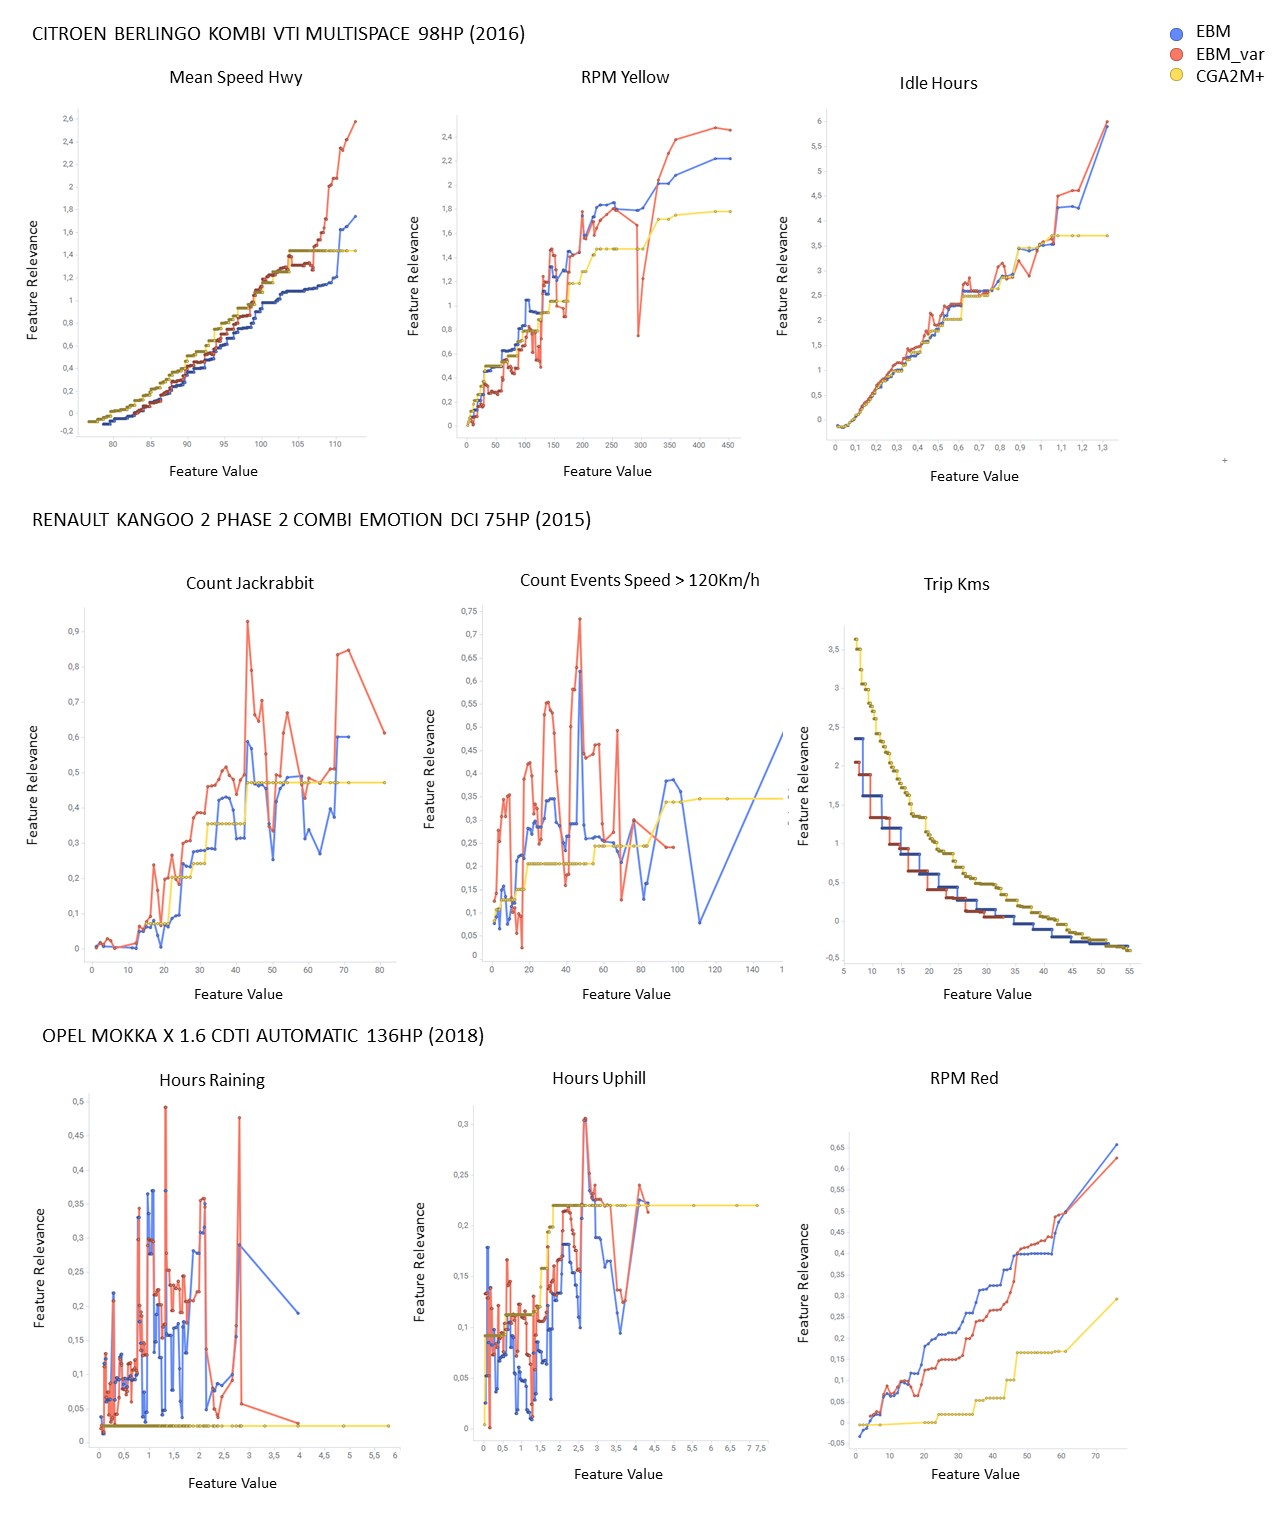
\includegraphics[width=\textwidth]{figures/chapter6_LucaFleet/PairplotComparison.jpg}
  \end{tabular} 
  \caption{Pairplot with the relevance-values for several features considering data points for some vehicle's models only, and using the data set of D1 (without applying the monotonicity filtering in EBM and EBM\_var).\label{fig:ch6-PairplotComparison}}
\end{figure*}

Extending the analysis to the other data sets, and focusing on the outliers only, we get the results shown in \hyperref[table:ch6-Fuel-Saved-Explained]{Table} \ref{table:ch6-Fuel-Saved-Explained}. We see how CGA2M+ still covers less fuel (in L) than EBM\_var for all data sets except for the smallest ones (D8 and D9). \textbf{On average, the fuel reduced among the largest data sets by EBM\_var final explanations is over 38\%, and over 29\% with CGA2M+.}

However, applying the monotonicity constraints over EBM and EBM\_var leads to a scenario where CGA2M+ covers more fuel than either EBM or EBM\_var, except for D1. This shows that if there is a need to \textbf{ensure the monotonicity of the feature explanation output}, and specially if the fleet size is not high enough, it is \textbf{better to impose it during the model learning} (CGA2M+), than applying it post hoc (EBM or EBM\_var). 

% TODO: Meter aqui la ultima comparativa con la tabla monotonicity filter
This last aspect is clearly seen in \hyperref[table:annex-xai-metrics-contrast-mono]{Table} \ref{table:annex-xai-metrics-contrast-mono}, where we show the XAI metrics after applying the monotonicity filter in EBM and EBM\_var (and with respect to the same CGA2M+ metric values). On general terms, CGA2M+ provides better results in all fleet sizes (though for \textit{precision} and \textit{contrastiveness} metrics the results are more similar). We also see that the filter penalizes more EBM\_var than EBM (since the monotonicity degree is higher in EBM). This points to two possible scenarios. When there is no need to ensure the monotonicity degree at every feature level (e.g., when the explanations are at a global level for profiles like fleet managers), EBM\_var is a good choice. However, when there is a need for ensuring the monotonicity within the individual explanations (e.g., for fleet operators), it is better to ensure it during the model's learning (CGA2M+), than afterwards. 

\begin{table}[h!]
\centering
\resizebox{420pt}{!}{%
\begin{tabular}{@{}lllllllll@{}}
\toprule
\textbf{\begin{tabular}[c]{@{}l@{}}Data \\ set\end{tabular}} & \textbf{Method} & \textbf{N points} & \textbf{\begin{tabular}[c]{@{}l@{}}Points\\ Expl. (\%)\end{tabular}} & \textbf{\begin{tabular}[c]{@{}l@{}}Fuel\\ Used (L)\end{tabular}} & \textbf{\begin{tabular}[c]{@{}l@{}}Fuel\\ Saved (L)\end{tabular}} & \textbf{\begin{tabular}[c]{@{}l@{}}Fuel\\ Saved (\%)\end{tabular}} & \textbf{\begin{tabular}[c]{@{}l@{}}Fuel Expl.\\ Monotonic (\%)\end{tabular}} & \textbf{\begin{tabular}[c]{@{}l@{}}Fuel Saved\\ Monotonic (\%)\end{tabular}} \\ \midrule
D1 & EBM & 5770 & 74 & 28599 & 6200 & 22 & 70 & 18 \\
D1 & EBM\_var & 5770 & 74 & 28599 & 6925 & 24 & 68 & 16 \\
D1 & monoGAM & 5770 & 70 & 28599 & 4629 & 16 & 70 & 16 \\
D2 & EBM & 1809 & 99 & 23139 & 10005 & 43 & 99 & 37 \\
D2 & EBM\_var & 1809 & 99 & 23139 & 11986 & 52 & 97 & 38 \\
D2 & monoGAM & 1809 & 99 & 23139 & 9710 & 42 & 99 & 42 \\
D3 & EBM & 10475 & 61 & 260152 & 36319 & 14 & 56 & 5 \\
D3 & EBM\_var & 10475 & 61 & 260152 & 46135 & 18 & 56 & 7 \\
D3 & monoGAM & 10475 & 60 & 260152 & 40853 & 16 & 60 & 16 \\
D4 & EBM & 1915 & 65 & 14301 & 1932 & 14 & 58 & 7 \\
D4 & EBM\_var & 1915 & 71 & 14301 & 2622 & 18 & 62 & 10 \\
D4 & monoGAM & 1915 & 69 & 14301 & 2175 & 15 & 69 & 15 \\
D5 & EBM & 724 & 43 & 6816 & 801 & 12 & 42 & 10 \\
D5 & EBM\_var & 724 & 43 & 6816 & 936 & 14 & 43 & 11 \\
D5 & monoGAM & 724 & 42 & 6816 & 763 & 11 & 42 & 11 \\
D6 & EBM & 2002 & 96 & 11157 & 3386 & 30 & 91 & 18 \\
D6 & EBM\_var & 2002 & 98 & 11157 & 4545 & 41 & 93 & 22 \\
D6 & monoGAM & 2002 & 95 & 11157 & 4047 & 36 & 95 & 36 \\
D7 & EBM & 942 & 58 & 41437 & 5995 & 14 & 48 & 8 \\
D7 & EBM\_var & 942 & 57 & 41437 & 6066 & 15 & 41 & 8 \\
D7 & monoGAM & 942 & 21 & 41437 & 4373 & 11 & 21 & 11 \\
D8 & EBM & 349 & 82 & 3164 & 333 & 11 & 69 & 4 \\
D8 & EBM\_var & 349 & 82 & 3164 & 368 & 12 & 65 & 4 \\
D8 & monoGAM & 349 & 92 & 3164 & 1144 & 36 & 92 & 36 \\
D9 & EBM & 10 & 100 & 471 & 44 & 9 & 80 & 3 \\
D9 & EBM\_var & 10 & 100 & 471 & 37 & 8 & 60 & 2 \\
D9 & monoGAM & 10 & 50 & 471 & 70 & 15 & 50 & 15 \\ \bottomrule
\end{tabular}%
}
\caption{Vehicle-dates (N data points) with anomalous fuel consumption explained by the different XAI models on the different fleets, together with the potential fuel saved (L and \%) with the recommendations.}
\label{table:ch6-Fuel-Saved-Explained}
\end{table}

\newpage
\section{Conclusion}\label{sec:ch6-conclusion}
We have proposed a complete process for explainable unsupervised anomaly detection in the fuel consumption of the vehicles of a fleet. Anomalies are explained using Explainable Artificial Intelligence (XAI) techniques and based on the feature relevance of several features that may impact in the fuel usage. The explanations take into account domain knowledge expressed through business rules and expressed through recommendations that are adjusted depending on two different user profiles that will use them: fleet managers and fleet operators. The process is evaluated using real-world data gathered from telematics devices connected to several industry fleets.

We have also evaluated different possibilities for building a surrogate model that infers the relationships between the input data and the predicted fuel consumption, in order to explain later how anomalous fuel consumption could be reduced. For those surrogate models, we have used Generalized Additive Models with Explainable Boosting Machine (EBM), Constrained Generalized Additive 2 Model with Consideration of Higher-Order Interactions (CGA2M+), and a proposal with a variation over the original EBM algorithm. 

To compare the different surrogate model alternatives, we have performed evaluations regarding model performance (how well the model predicts the target feature), and XAI metrics, that compare the explanations generated in terms of representativeness, fidelity, stability, contrastiveness and consistency with apriori beliefs. 

The evaluations show that all interpretable models yield good results in terms of model performance. For the XAI metrics, particularly for the consistency with apriori beliefs, we see that the three models yield good results by themselves and are able to provide appropriate recommendations over 80\% of the anomalous instances, that could potentially lead to fuel reductions of up to 38\% on average on large fleets. The XAI metrics are also used for comparing the models between them, where we saw that in general, both CGA2M+ and EBM\_var provide similar or better results than EBM, while respectively solving monotonicity problems and considering the vehicle model and route type information for adjusting the explanations.

Along with that, we have verified that the explanations are indeed aligned to prior domain knowledge regarding the factors that impact on vehicle fuel consumption. We have also shown how model performance is acceptable even after applying restrictions in the model for aligning the output to prior domain knowledge. Following this, we have also seen that the model performance is similar to that of unconstrained SOTA blackbox models.

With that, the work presented in this chapter serves for evaluating both \textbf{H1} and \textbf{H2}, described in \hyperref[sec:Hypotheses]{Section} \ref{sec:Hypotheses}. Regarding H1, we have applied an XAI approach for explaining the output of an unsupervised anomaly detection algorithm and we have compared the resulting explanations through XAI-specific metrics. For the case of H2, we have combined those XAI approaches with prior domain knowledge, showing that this does not penalize significantly the model performance, and we have analyzed how the final explanations are aligned to that prior knowledge.
Thus, this chapter offers a complete evaluation of the sub-hypothesis that are beneath the main hypothesis of this thesis.

%\subsection{Potential impact}\label{subsec:ch6-conclusion-potential-impact}
%The previous information showed what variables are impacting on the fuel consumption of individual vehicles, and how much fuel could be reduced by acting upon them through the explanations provided. This information is useful for having a full view over the whole fleet and seeing the extra fuel consumption that it is taking place because of those factors. Even more, we can focus on specially actionable factors, such as driving behaviour, in order to see the impact on the fuel consumption due to the driving style. \hyperref[table:ch6-ExtraFuelPerMonth]{Figure} \ref{table:ch6-ExtraFuelPerMonth} shows the fuel consumption on each of the fleets over the four months considered, together with the extra fuel consumption from driving behaviour, and the extra fuel consumption due to the remaining factors.

%\begin{figure}[h!]
%\centering
% \begin{tabular}{c@{\qquad}c@{\qquad}c}
%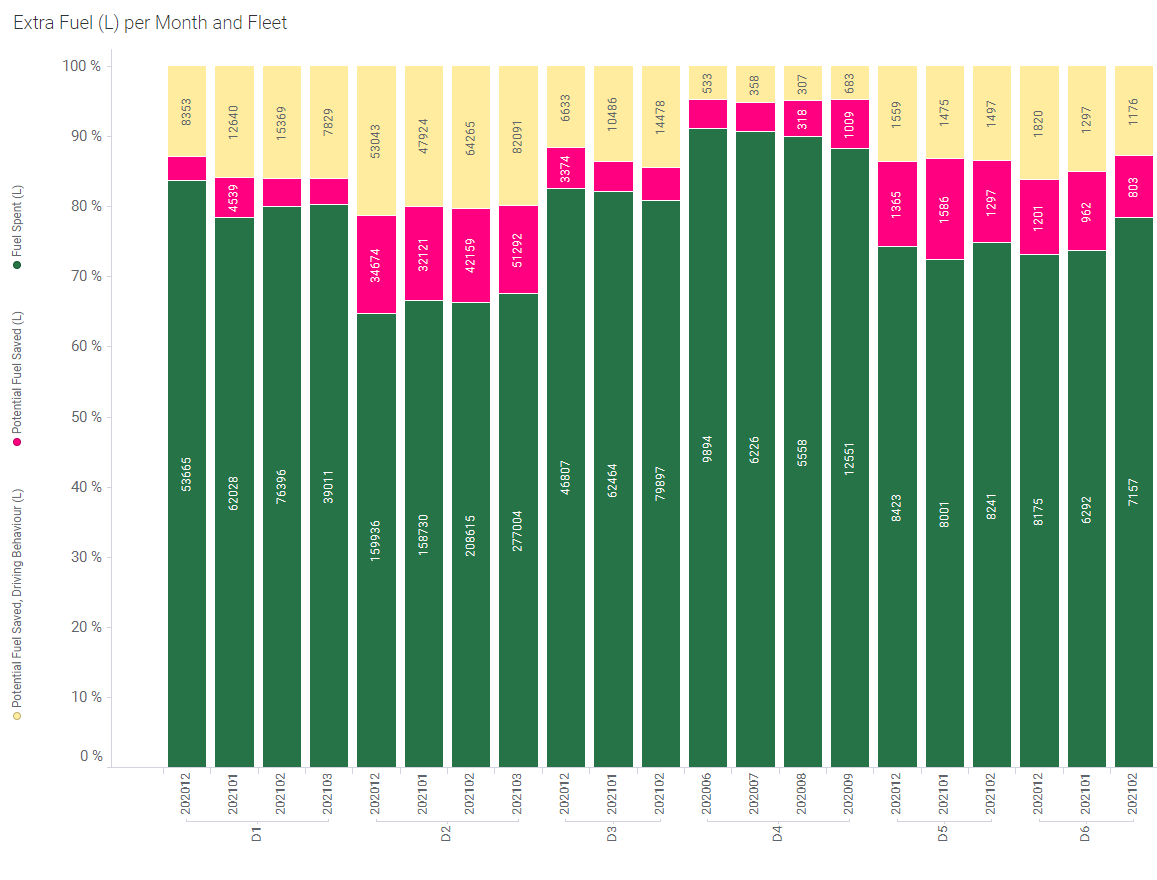
\includegraphics[width=430pt, height=550pt, %keepaspectratio]{figures/chapter6_LucaFleet/ExtraPerMonthFleet.PNG}
%  \end{tabular} 
%  \caption{Monthly fuel consumption (L) for each fleet over the different months, along with the part of that fuel that corresponds to the extra fuel due to driving behaviour, together with the extra fuel from the remaining factors. This is considering both inliers and outliers.  \label{table:ch6-ExtraFuelPerMonth}}
%\end{figure}

%Focusing on D1 (since it is the fleet with more information and that provided better results) and for all data points with extra fuel (even if they are outliers per se), we see that the relative impact of all the features is between 16\% and 22\%, and for driving behaviour only, it is between 13\% and 16\%. Taking as an example the month of February, we see that there are 15546 extra litres spent due to driving behaviour. Reducing it would have a positive impact both in the expenses from the fleet, as well as in the environment. Since the vehicles from D1 are mostly diesel, using the conversion to CO2 from \parencite{DieselLitresTOCo2}, where 2.67633 Kg of CO2 are emitted per liter of diesel spent, the extra CO2 emissions in one month due to driving behaviour is between 22330 and 41085 Kg.